\documentclass[aspectratio=169]{beamer}

% Packages
\usepackage{amsthm}        % For theorems
\usepackage{amsmath}       % For math
\usepackage{luatexja}      % For Japanese
\usepackage{booktabs}      % For formal tables
\usepackage{mathtools}
\usepackage{amssymb}       % For checkmark
\usepackage{ulem}          % For strikeout
\usepackage[dvipsnames]{xcolor} % For colors (i.e. ForestGreen)
\usepackage[noend]{algpseudocode}
\usepackage[backend=biber,
            style=alphabetic,
            sorting=none
            ]{biblatex}    % For bibliography
\usepackage{tikz}          % For figures
\usepackage{multirow}      % For multirow in tables
\usetikzlibrary{arrows.meta,
                chains,
                positioning}
\addbibresource{references.bib}

% Beamer settings
\setbeamertemplate{theorems}[numbered]
\addtobeamertemplate{theorem begin}{\normalfont}{}
\newtheorem*{theorem*}{Theorem}
\newtheorem*{sproof}{Sketch of the proof.}
\newtheorem{remark}{Remark}
\newtheorem{algorithm}{Algorithm}
\newtheorem{scheme}{Scheme}
\newtheorem{conjecture}{Conjecture}

\newcommand{\info}[1]{\textcolor{ForestGreen}{#1}}

% Theme
\usetheme{metropolis}
\usecolortheme{default}
\metroset{block=fill}

% Fonts
\setbeamerfont{title}{size=\large,series=\bfseries}
\setbeamerfont{theorem}{shape=\upshape}
\usefonttheme{professionalfonts}
\usefonttheme{structurebold}
\setbeamerfont{title}{size=\LARGE}
\setbeamerfont{date}{size=\small}
\setbeamerfont{frametitle}{size=\large,series=\bfseries}
\usepackage[T1]{fontenc}
\usepackage{mlmodern}
\usepackage{luatexja-otf}
\renewcommand{\kanjifamilydefault}{\gtdefault}
\renewcommand{\familydefault}{\sfdefault}

% Metadata
\title{3.4 ナップサック問題に対する FPTAS}
\subtitle{近似アルゴリズム ―離散最適化問題への効果的アプローチ― pp.68--73}
\author{岡山 大輝}
\institute{兵庫県立大学大学院 情報科学研究科\textit{(ad25r010@guh.u-hyogo.ac.jp)}}
\date{June 30, 2025}

% \AtBeginSection[]
% {
%   \begin{frame}{目次}
%     \tableofcontents[currentsection]
%   \end{frame}
% }

\begin{document}

\begin{frame}
	\titlepage{}
\end{frame}

\begin{frame}{導入：ナップサック問題への招待}
	\structure{\alert{重さの上限}の中で\alert{価値の和を最大}にする組み合わせは？}
	\begin{figure}
		\centering
		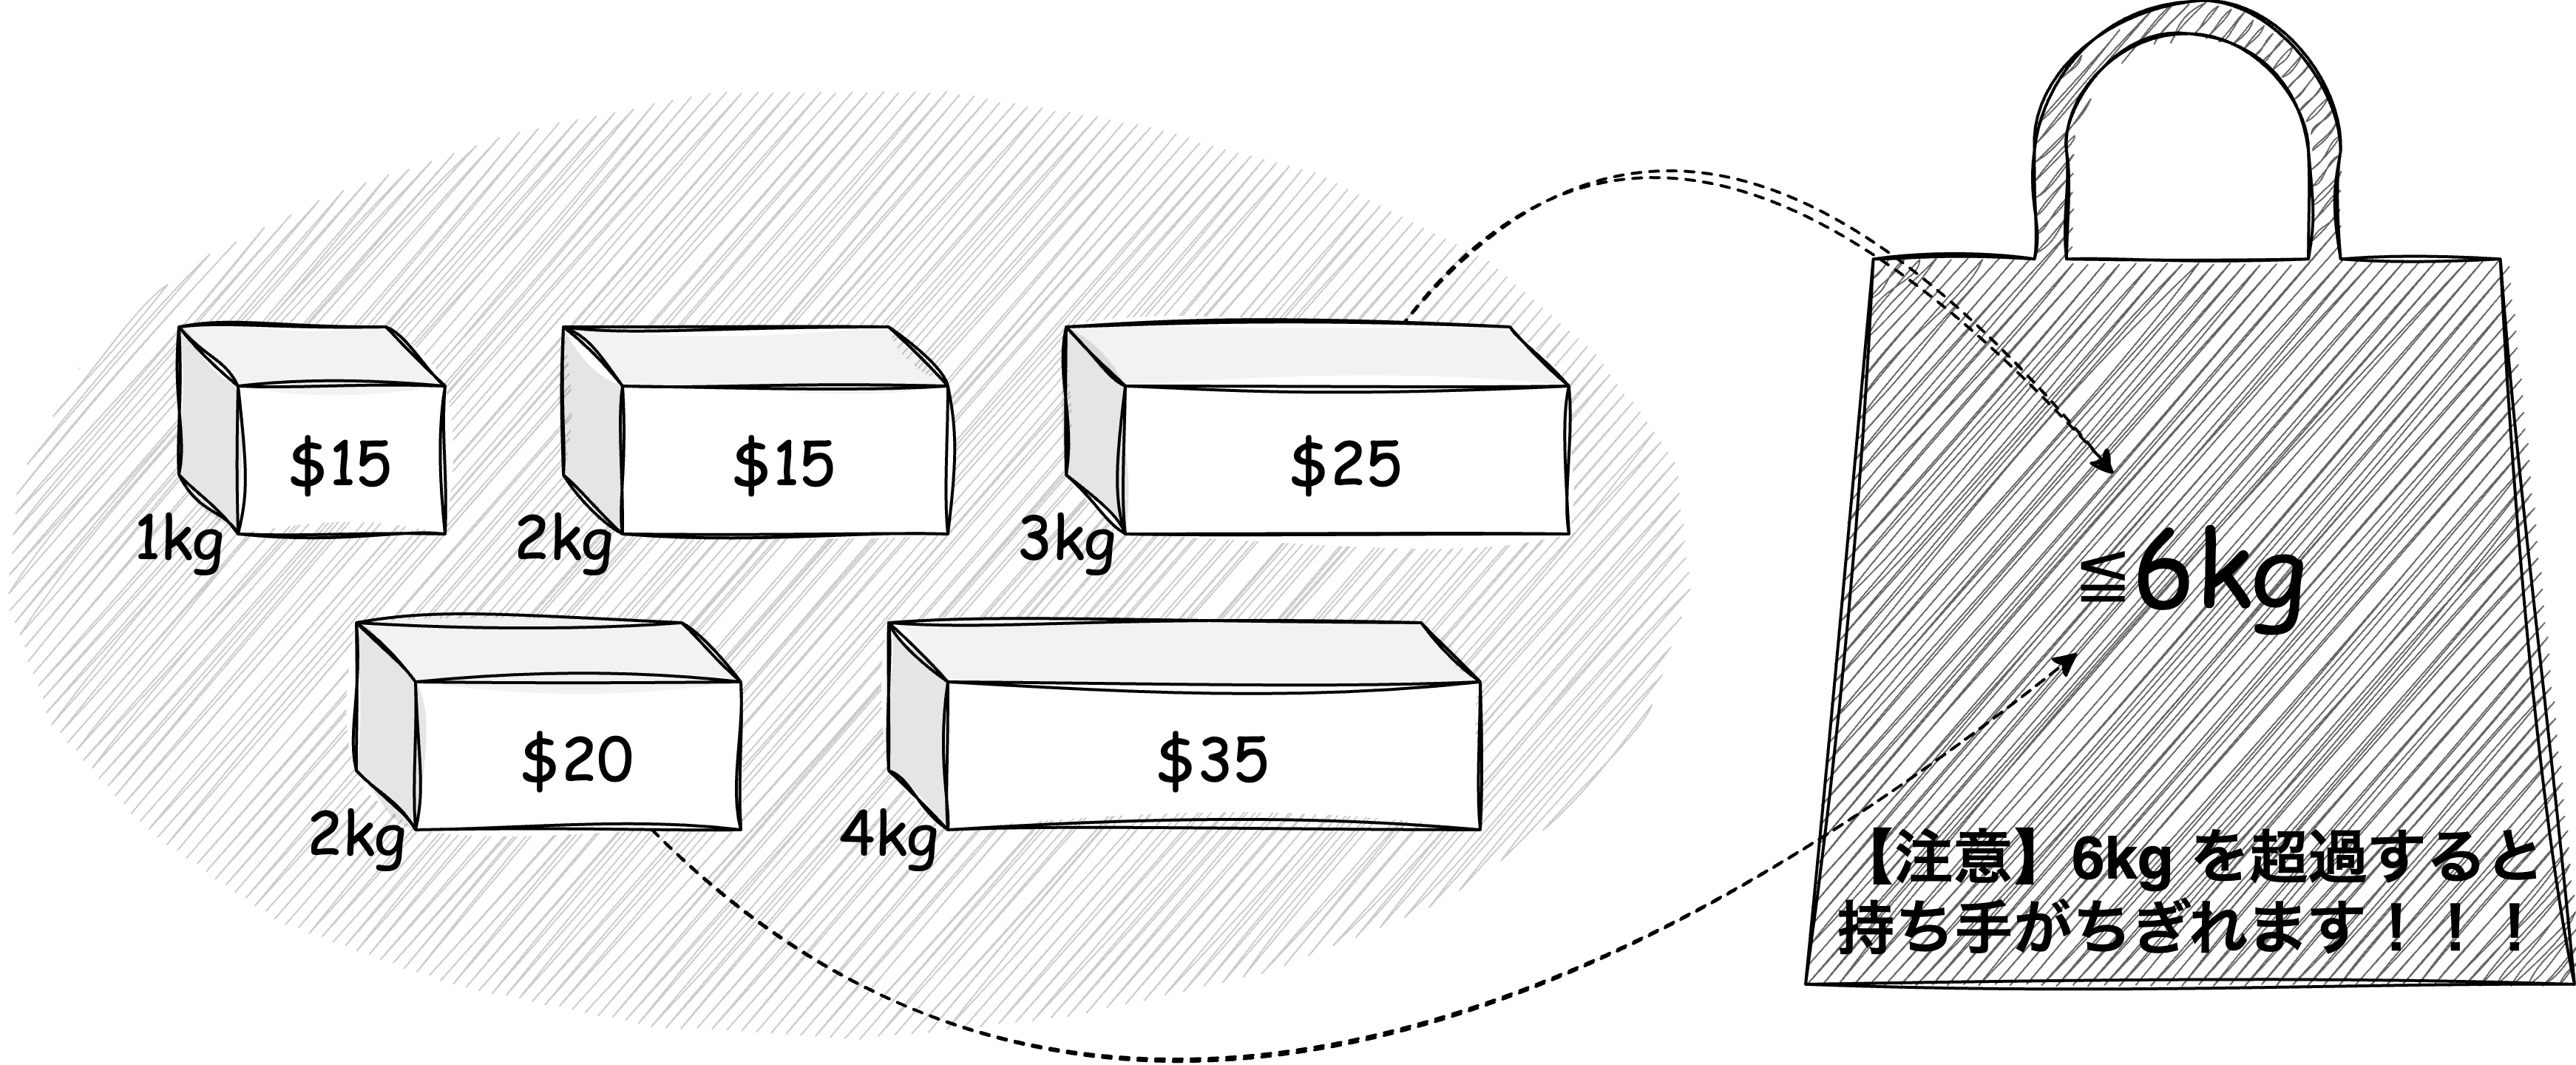
\includegraphics[width=1.0\textwidth]{figures/knapsack-problem.png}
	\end{figure}
\end{frame}

\begin{frame}{ナップサック問題}
	\vskip 1em

	\begin{problem}[ナップサック問題]
	\begin{itemize}
		\leftskip 3em
		\item[Input: ] \(\boldsymbol{a}, \boldsymbol{c} \in \mathbb{Z}^n_{+}, b \in \mathbb{Z}_{+}\)
		\item[Output: ] \(\boldsymbol{x} \in \{0, 1\}^n\) such that
		      \[
			      \alert{\boldsymbol{a}^T \boldsymbol{x} \leq b} \quad \text{and} \quad \alert{\boldsymbol{c}^T \boldsymbol{x} \text{ is maximized.}}
		      \]
	\end{itemize}
	\end{problem}

	\begin{figure}
		\centering
		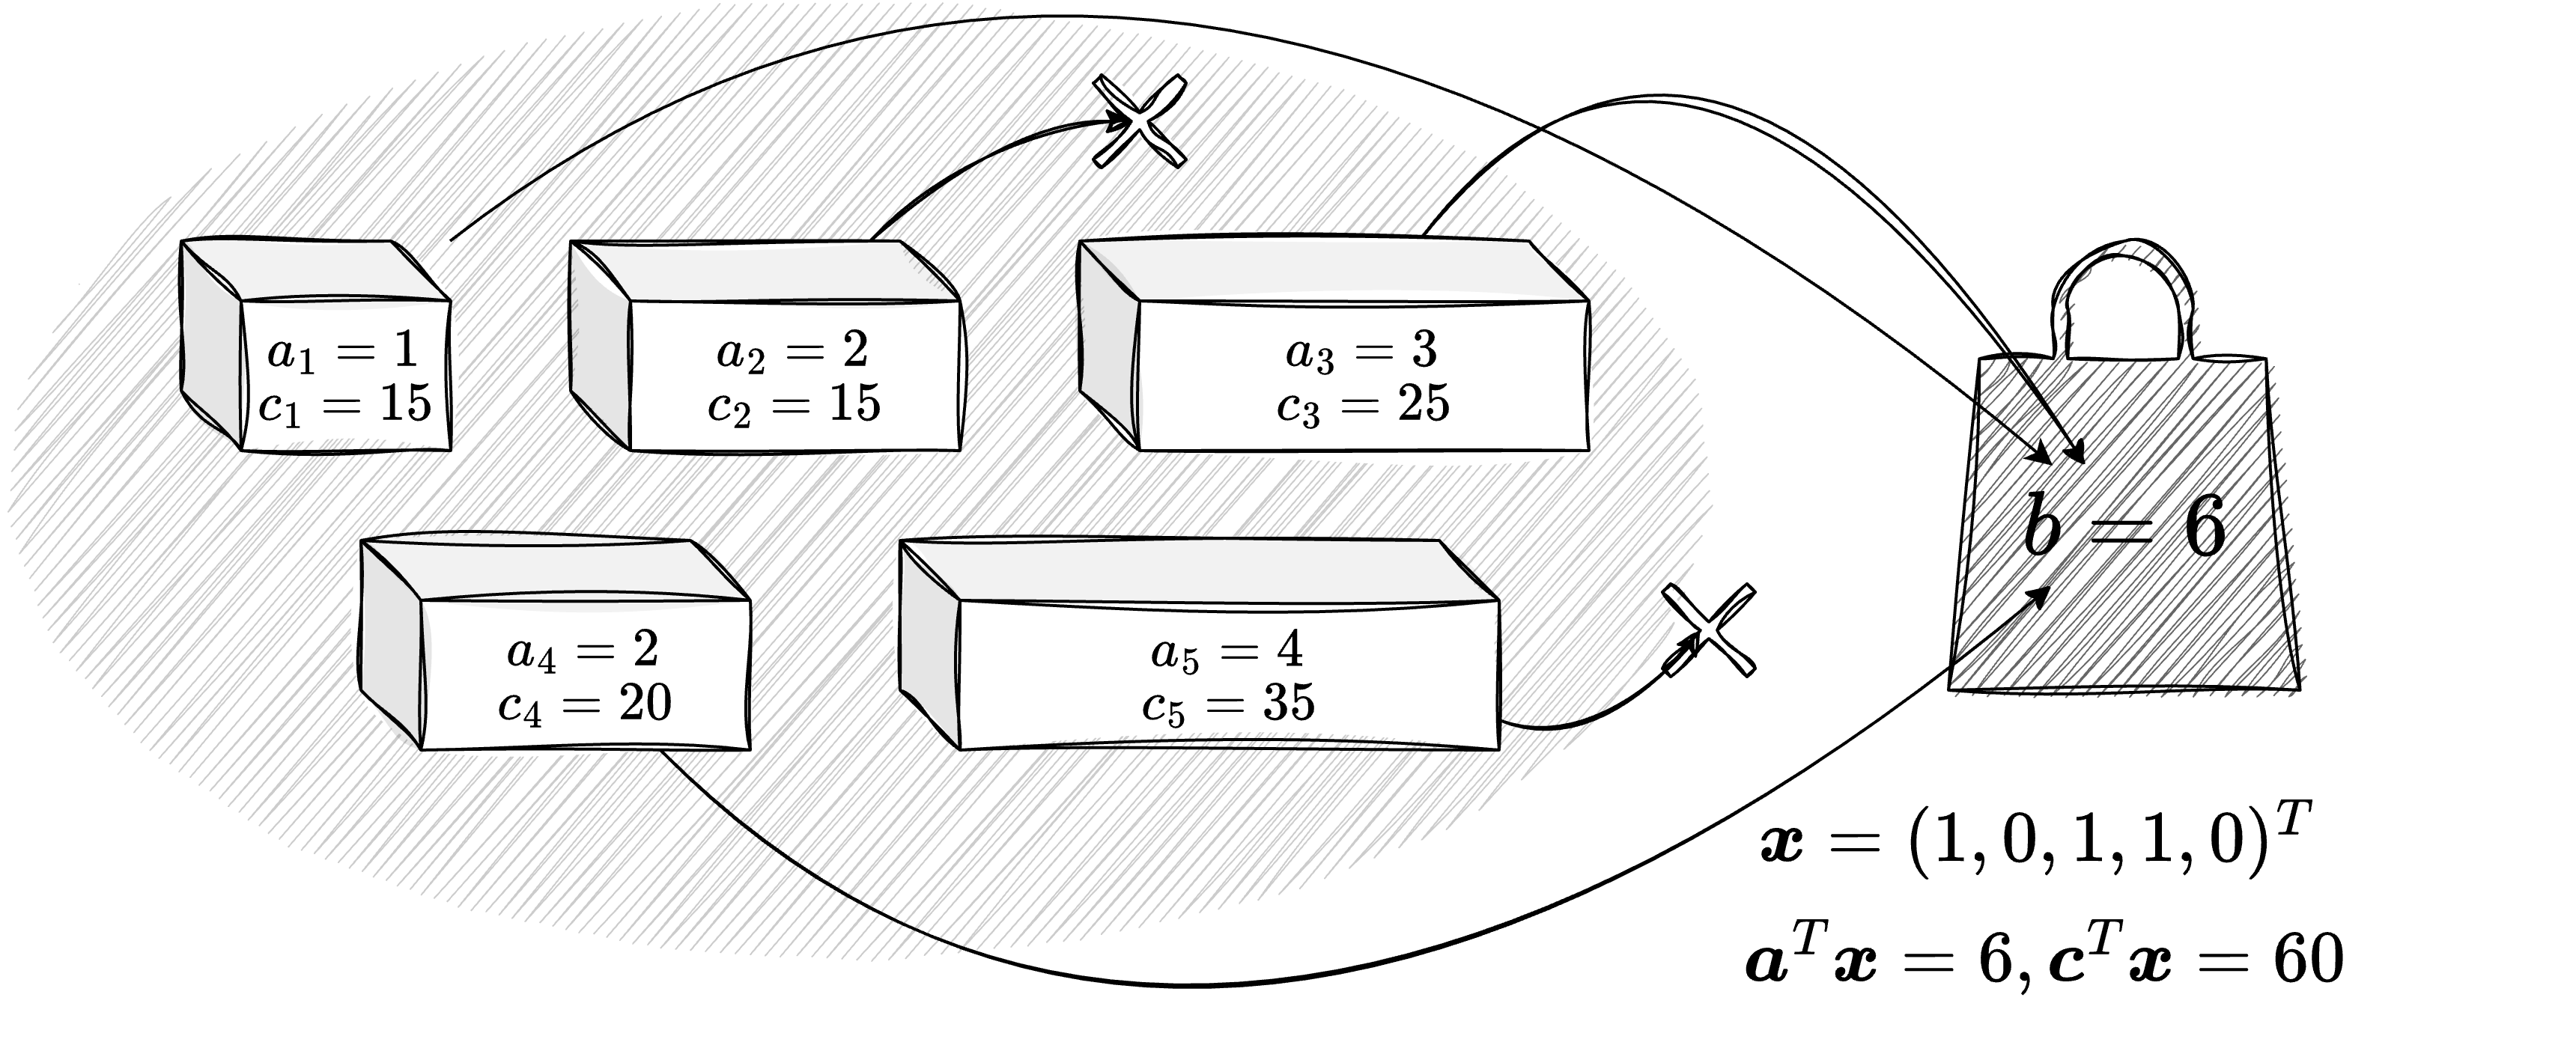
\includegraphics[width=0.75\textwidth]{figures/knapsack-problem-formally.png}
	\end{figure}
\end{frame}

\begin{frame}{ウォームアップ：ナップサック問題に対する貪欲的アルゴリズムの近似比}
	\vskip 0.5em

	\begin{algorithm}[貪欲的アルゴリズム]
		\begin{itemize}
			\item アイテムを\alert{単位価値 \(c_i / a_i\) の降順にソート}
			\item アイテムを順に選択し，ナップサックの容量を超えないように追加
		\end{itemize}
	\end{algorithm}

	\only<1>{

		\vskip 0.5em

		\begin{figure}
			\centering
			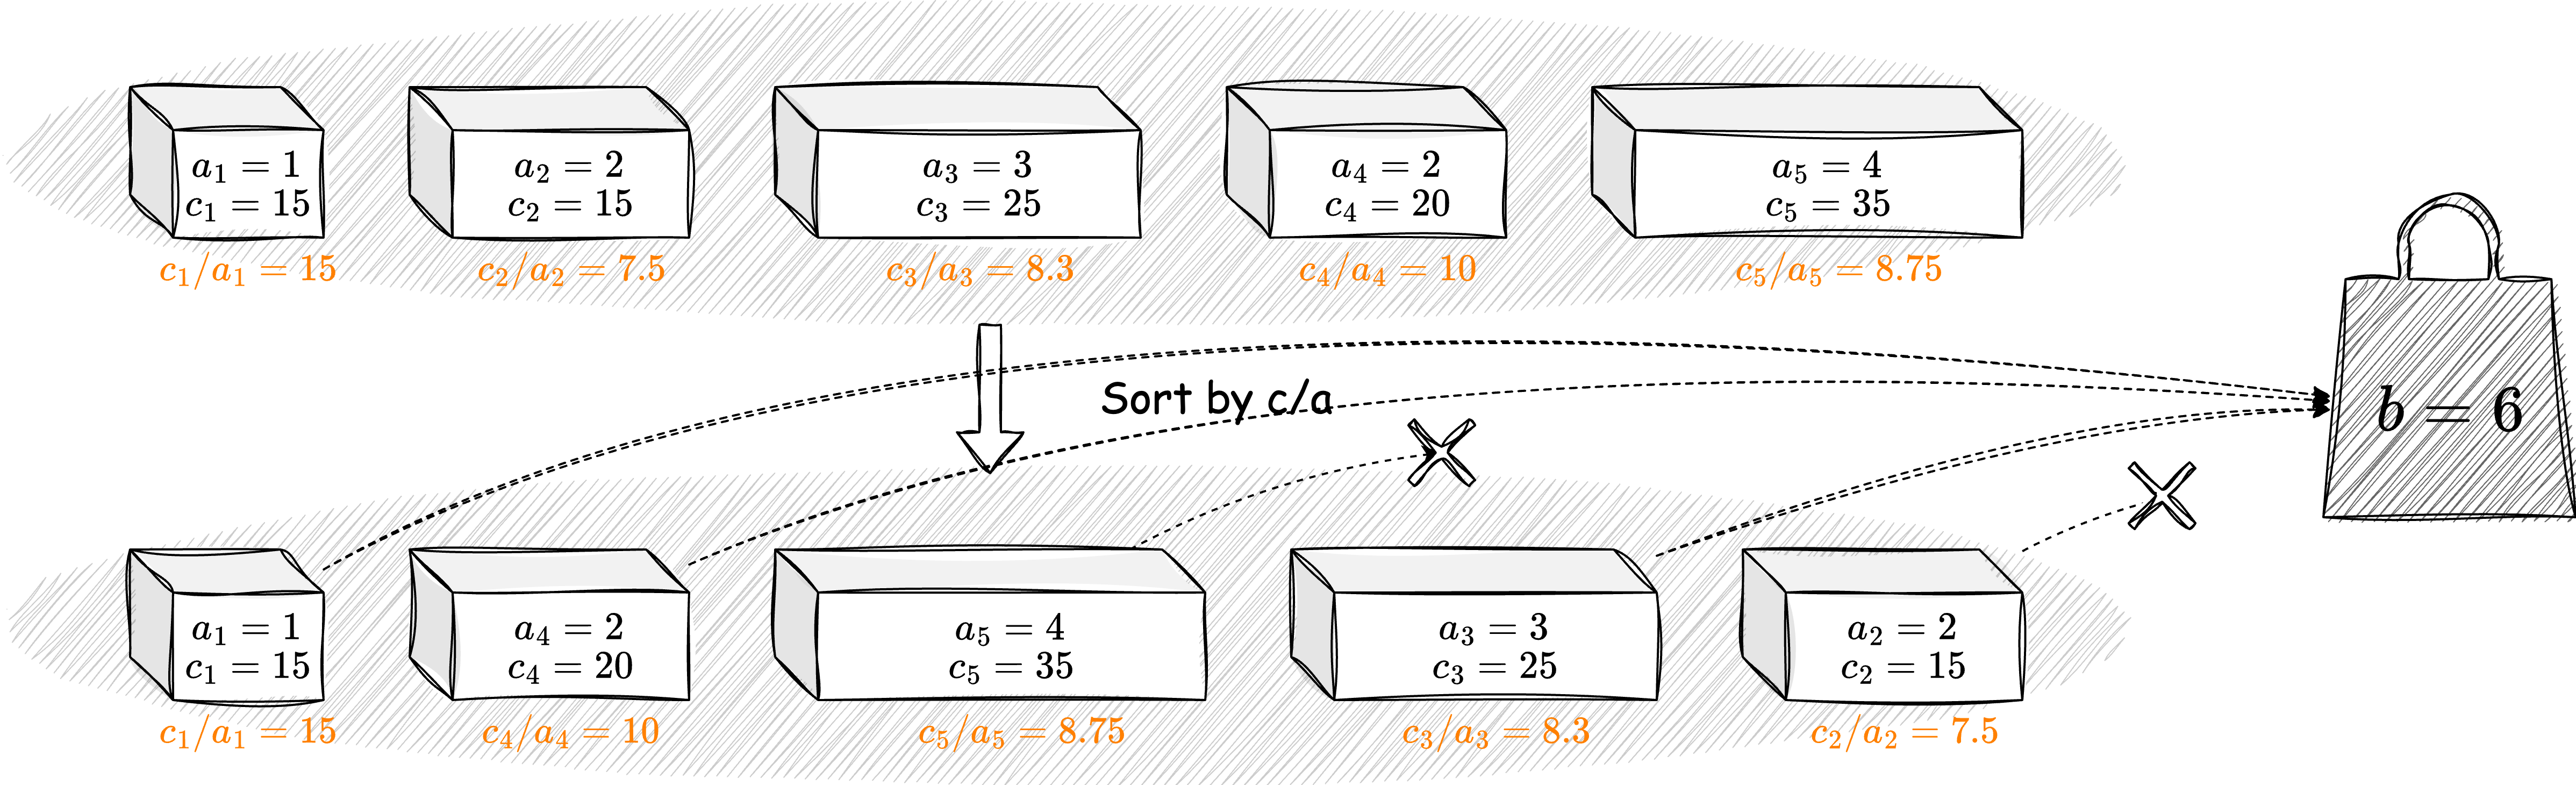
\includegraphics[width=1.0\textwidth]{figures/greedy.png}
		\end{figure}
	}
	\pause

	\begin{remark}[貪欲的アルゴリズムの近似比]
		いかなる正の定数 \(\delta < 1\) であっても，貪欲的アルゴリズムは\alert{近似保証 \(1 - \delta\) を達成できない}．
	\end{remark}

	\textbf{Proof.}
	任意に選択したナップサックのサイズ \(b \in \mathbb{Z}_+\) に対して，\(\boldsymbol{a} = (\alert{1}, b), \boldsymbol{c} = (\alert{b + 1}, b^2)\) と定める．
	単位価値が \(\boldsymbol{c} \oslash \boldsymbol{a} = (\alert{b + 1}, b)\) であることに注意すると，
	このインスタンスに対して貪欲的アルゴリズムが出力する解の近似率は，
	\[
		\frac{\alert{\textrm{ALG}}}{\textrm{OPT}} = \frac{\alert{b + 1}}{b^2} \xrightarrow[b \to \infty]{} 0
	\]
	となる．\qed

\end{frame}

\begin{frame}{振り返り：ナップサック問題に対する動的計画法}
	\vskip 0.5em

	\begin{theorem}[ナップサック問題の擬多項式時間アルゴリズム]
		ナップサック問題に対して，\alert{\(\mathcal{O}(n^2 C)\) 時間}で\alert{最適解}を求めるアルゴリズムが存在する．
		ただし，\(C = \max_i{c_i}\) とする．
	\end{theorem}

	\only<1>{
		\begin{figure}
			\centering
			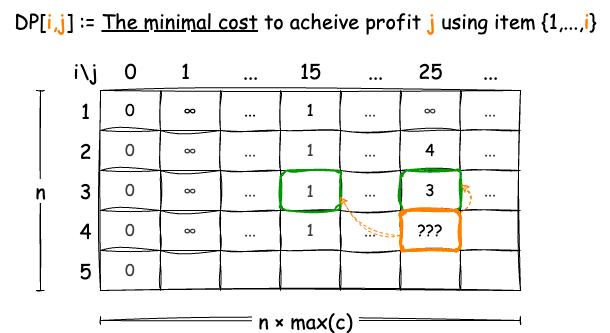
\includegraphics[width=1.0\textwidth]{figures/dp.png}
		\end{figure}
	}

	\only<2>{
		\begin{figure}
			\centering
			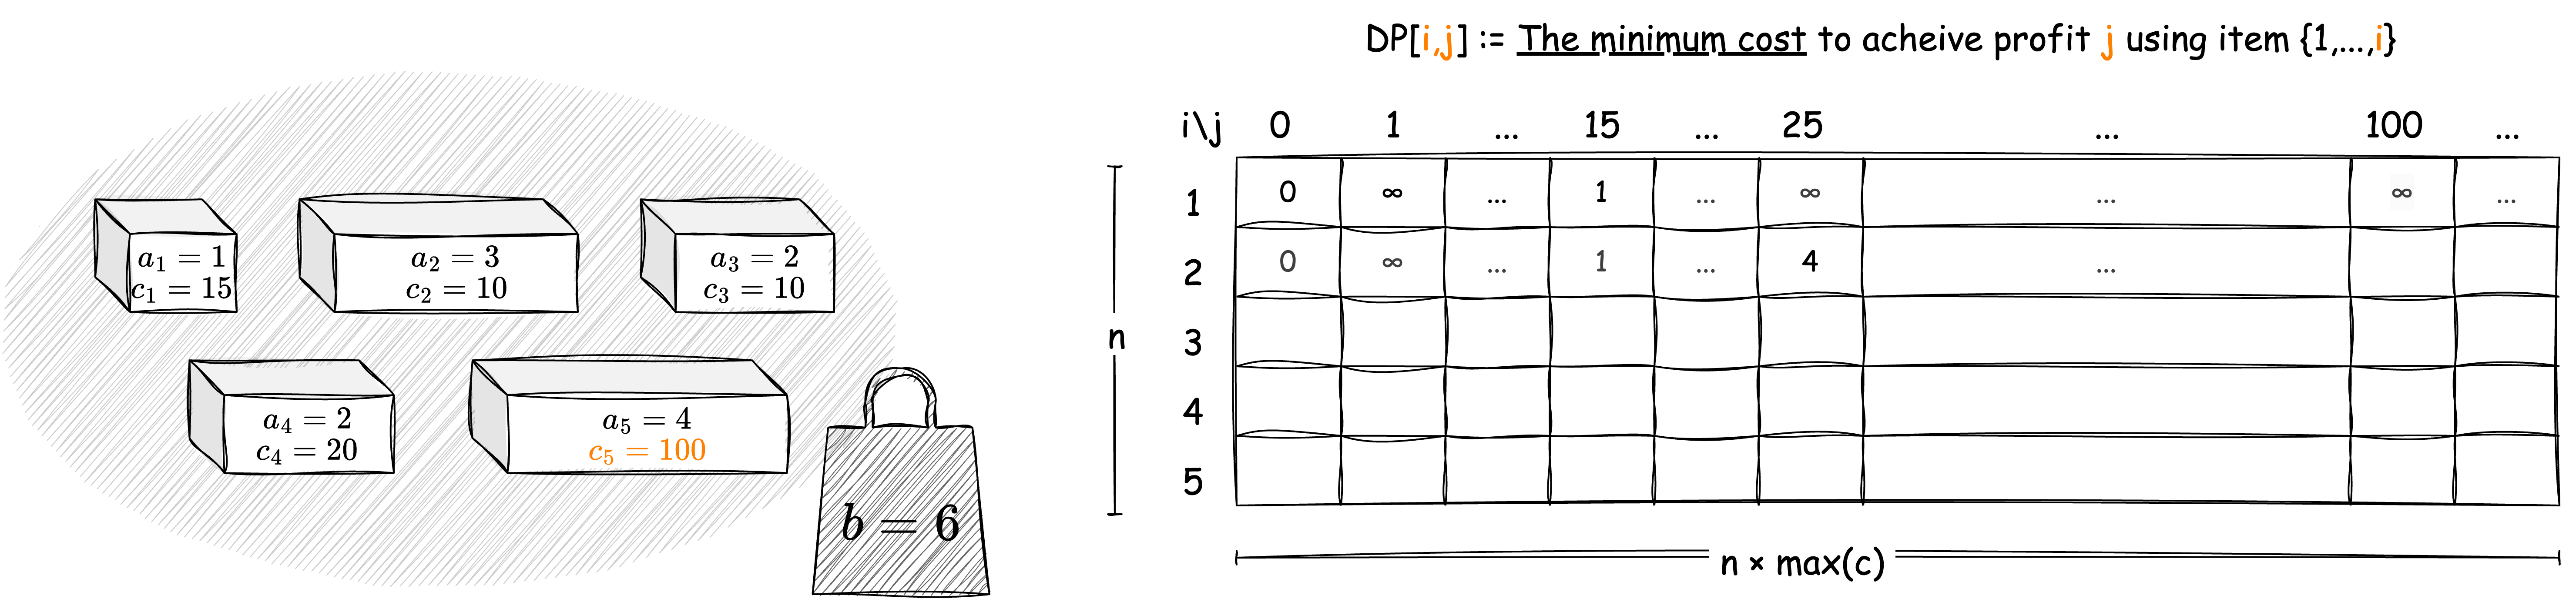
\includegraphics[width=1.0\textwidth]{figures/dp-long.png}
		\end{figure}
	}

	\only<3>{
		\begin{figure}
			\centering
			
\includegraphics[width=1.0\textwidth]{figures/dp-long-long.png}
		\end{figure}
	}
\end{frame}

\begin{frame}{本日のメイン：ナップサック問題に対する FPTAS}
	% \begin{block}{Key Idea}
	% 	\begin{itemize}
	% 		\item \(C = poly(n)\) のとき，\(n\) の多項式時間で最適解は求まる\footnote{\(C = \max_i{c_i}\)}
	% 		\item \(c_1, c_2, \ldots, c_n\) を適切にスケールダウンする
	% 	\end{itemize}
	% \end{block}

	\begin{theorem}[\alert{ナップサック問題の FPTAS}]
		ナップサック問題に対して，任意の正数 \(\varepsilon < 1\) に対し，\alert{\(\mathcal{O}(n^3/\varepsilon)\)} 時間で \alert{\((1 - \varepsilon)\)} 倍の近似解を求めるスキームが存在する．
	\end{theorem}

	\begin{scheme}
		\begin{itemize}
			\item 与えられた \(0 < \varepsilon < 1\) に対し，\alert{\(K = \varepsilon C / n\)} を定める\footnote{\(C (= \max_i{c_i})\) は商品の最大価値, \(n\) は商品の総数}
			\item 価値を \alert{\(c_i' = \lfloor c_i / K \rfloor\)} で修正する\footnote{このとき，\(c_i' \le \lfloor n / \varepsilon \rfloor\) になることに注意する}
			\item 修正価値のもとで，動的計画法を適用する
		\end{itemize}
	\end{scheme}
\end{frame}

\begin{frame}{スキームの動作例：\(\varepsilon = 0.3\) の場合 }
	\vskip 1em

	\only<1>{

		\begin{figure}
			\centering
			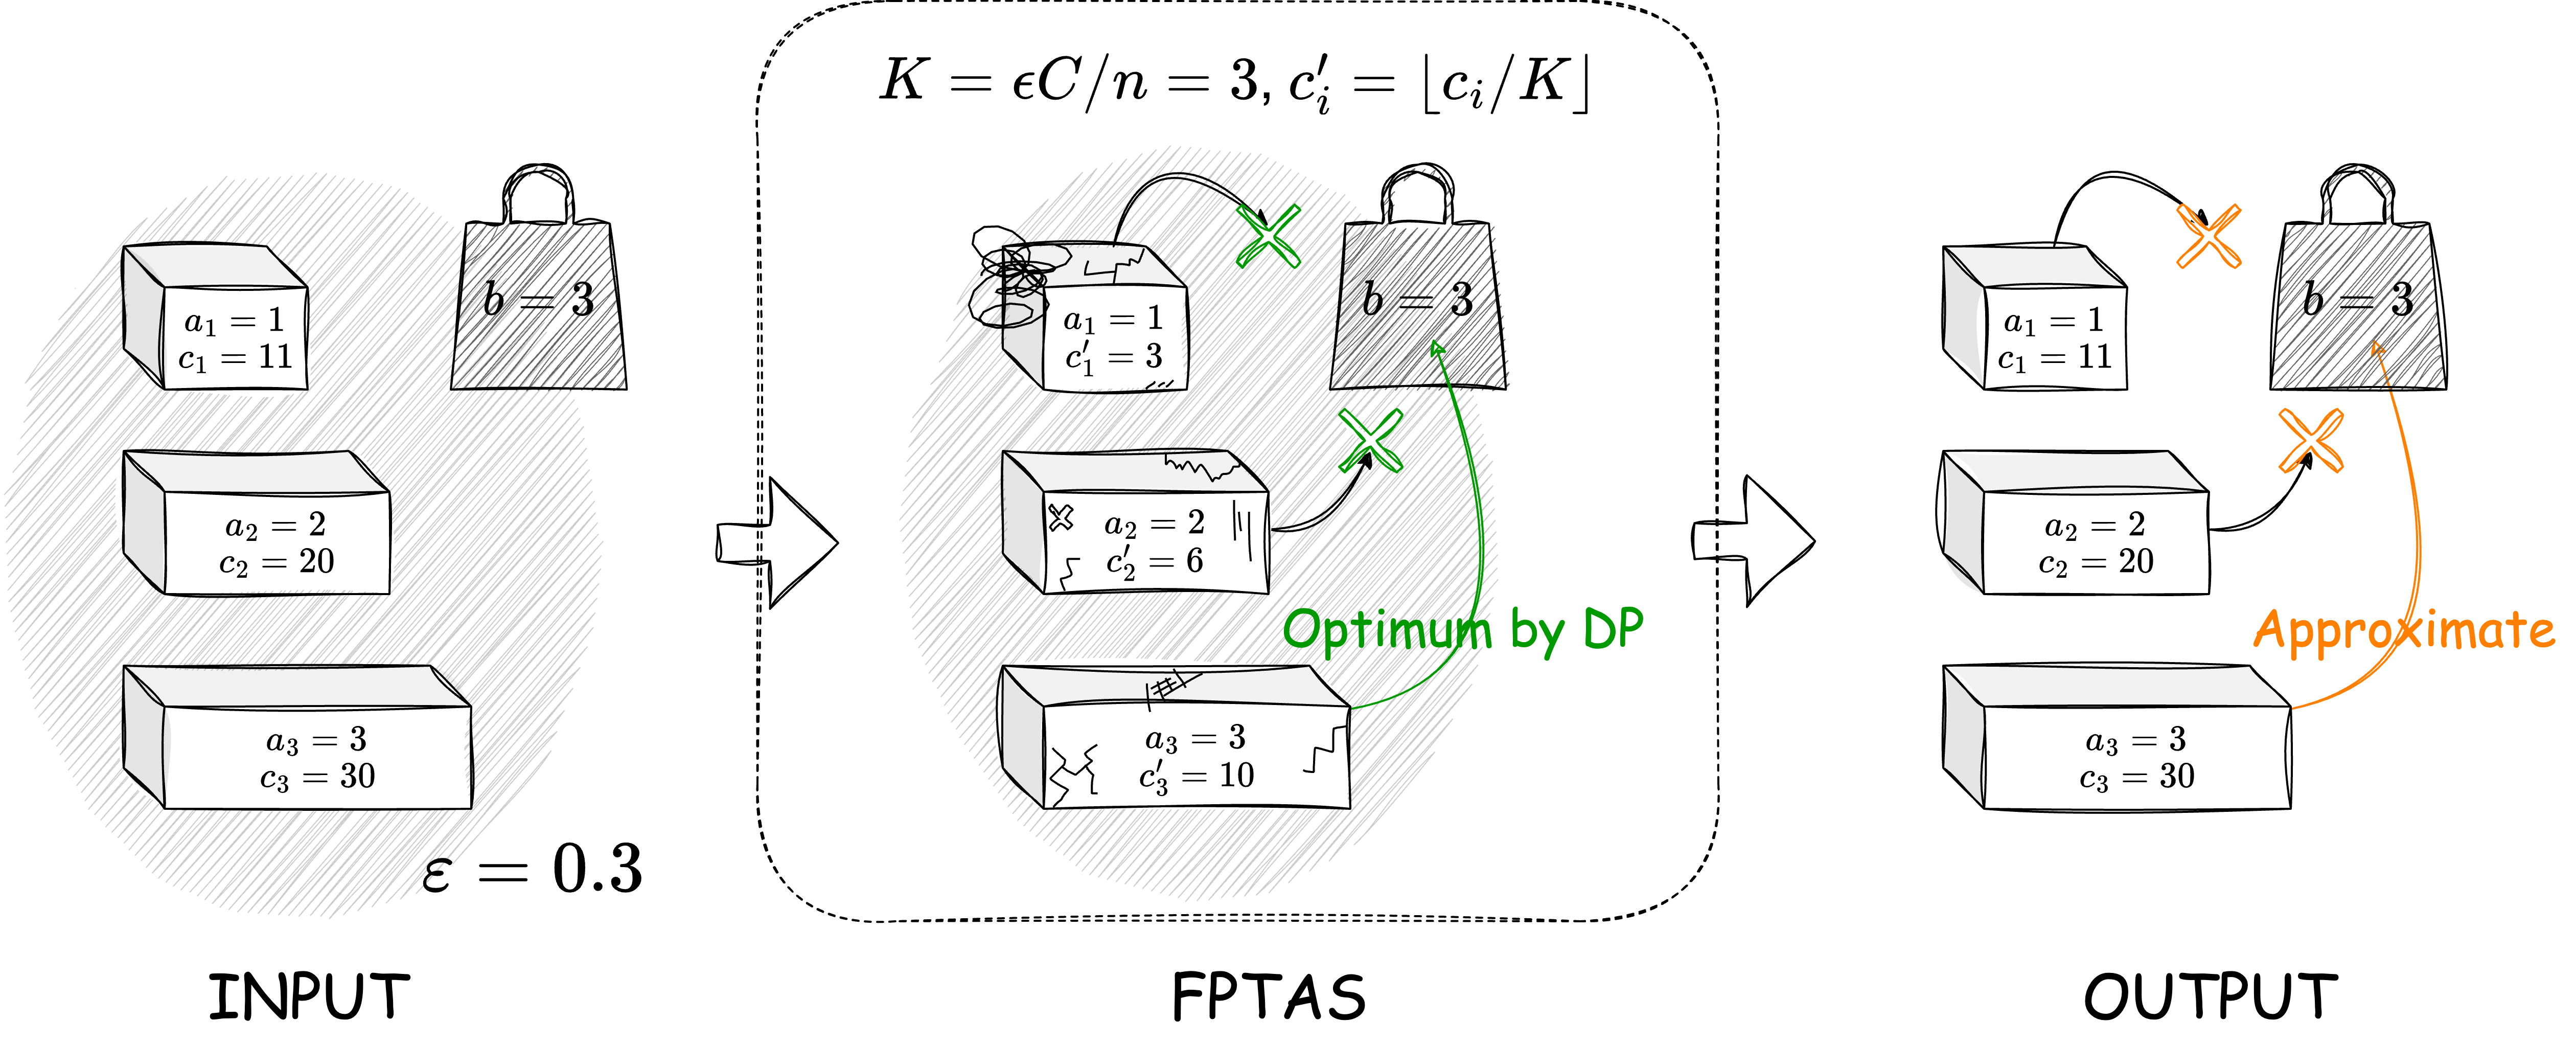
\includegraphics[width=1.0\textwidth]{figures/fptas.png}
		\end{figure}
	}

	\only<2>{
		\begin{figure}
			\centering
			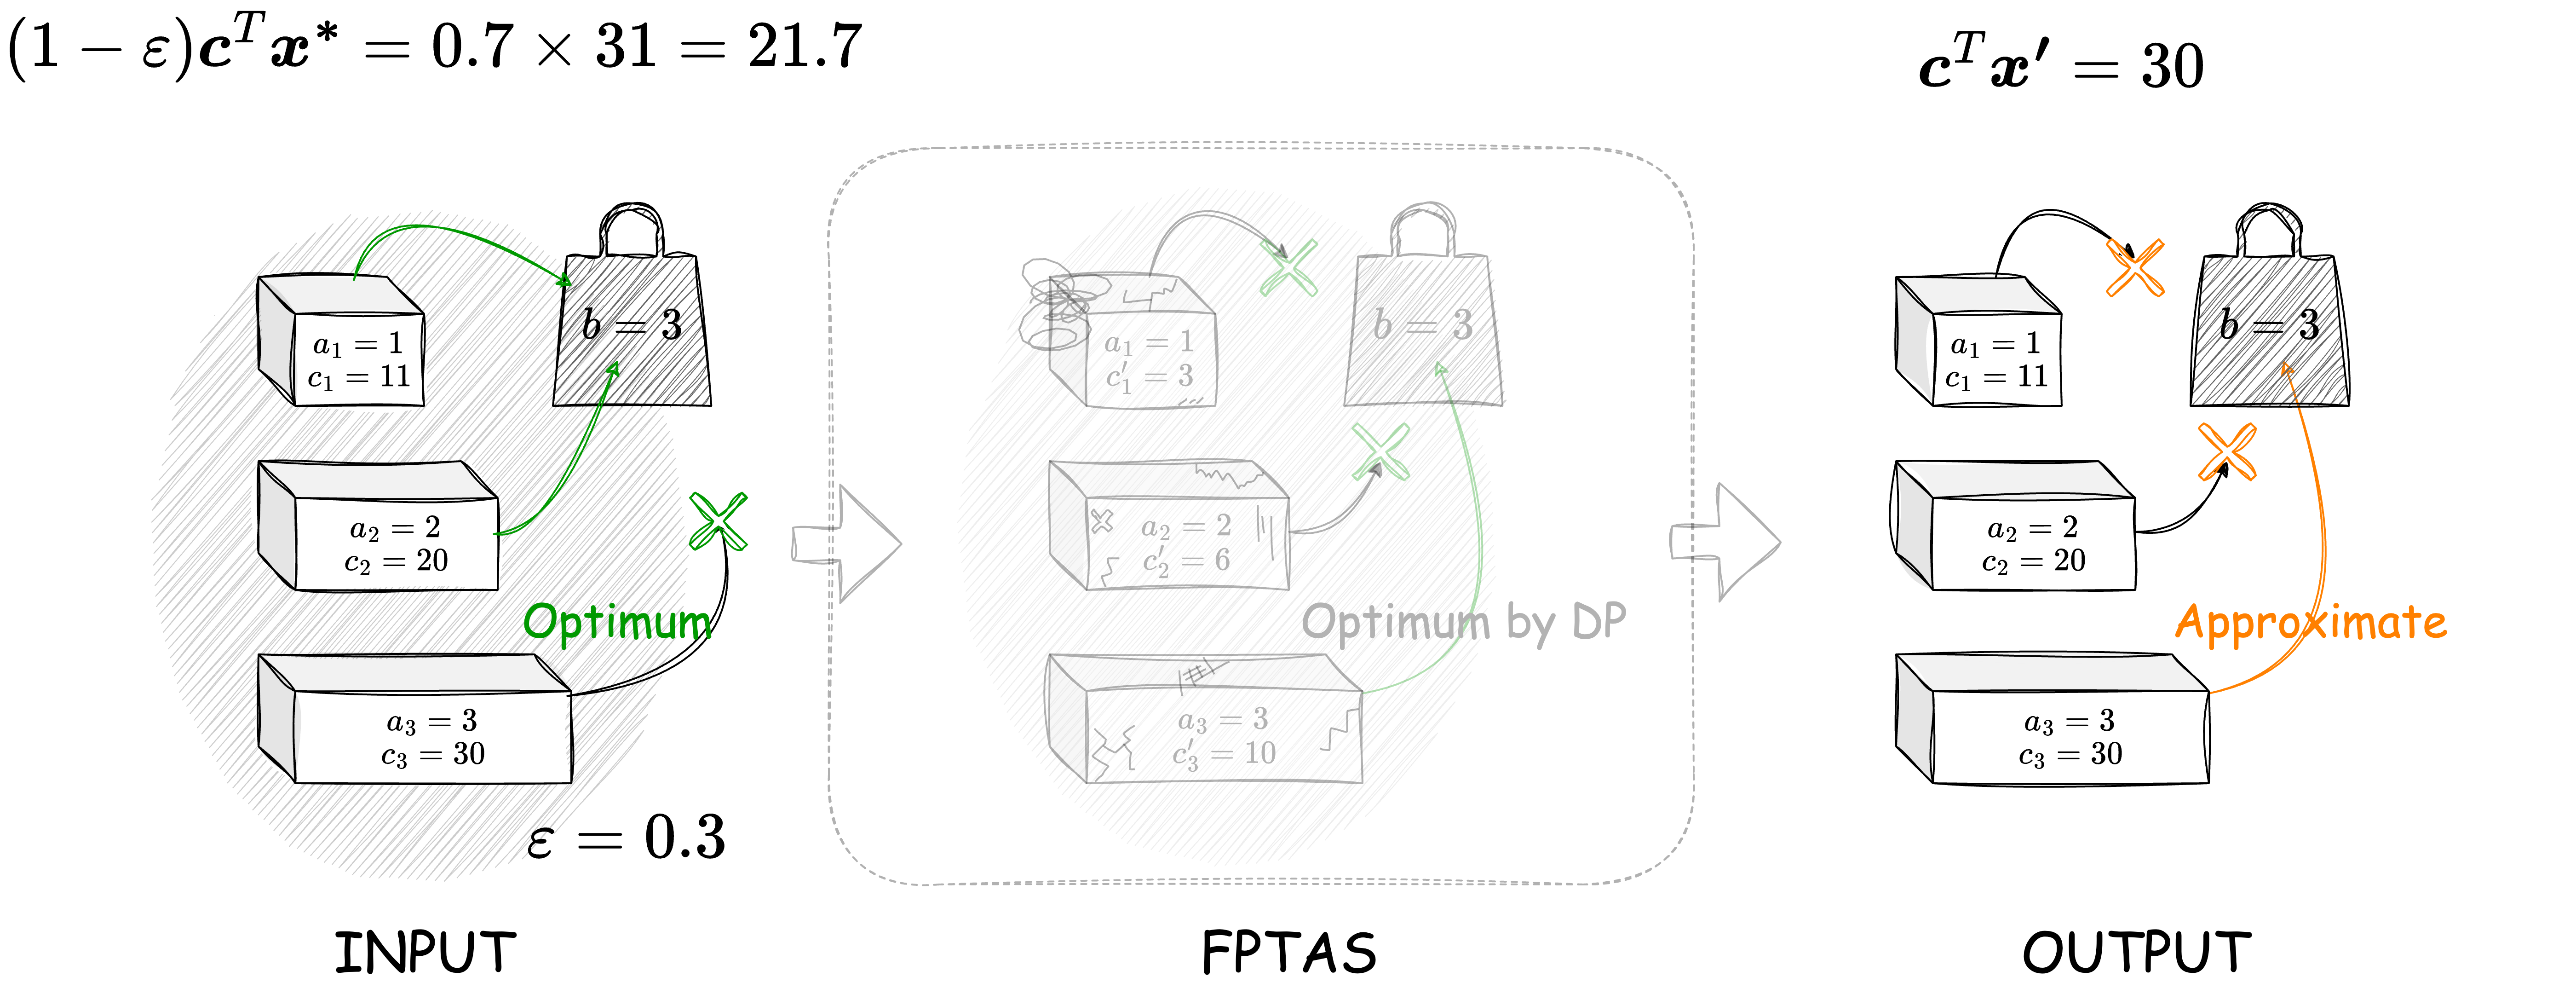
\includegraphics[width=1.0\textwidth]{figures/fptas-vs-optimal.png}
		\end{figure}
	}

	\pause

	\structure{なお，実際の最適解は \info{\(\boldsymbol{x}^* = (1, 1, 0)^T\)} で，このときの価値は \info{\(\boldsymbol{c}^T \boldsymbol{x}^* = 31\)} である．}

\end{frame}

\begin{frame}{スキームの近似保証}
	\vskip 1em

	\begin{lemma}[スキームの近似保証]
		スキームが出力する解 \(\boldsymbol{x'}\) は，次式を満たす．
		\[
			\alert{\boldsymbol{c}^T \boldsymbol{x'} \geq (1 - \varepsilon) \cdot{\boldsymbol{c}}^T \boldsymbol{x^*}}
		\]
	\end{lemma}

	\begin{figure}
		\centering
		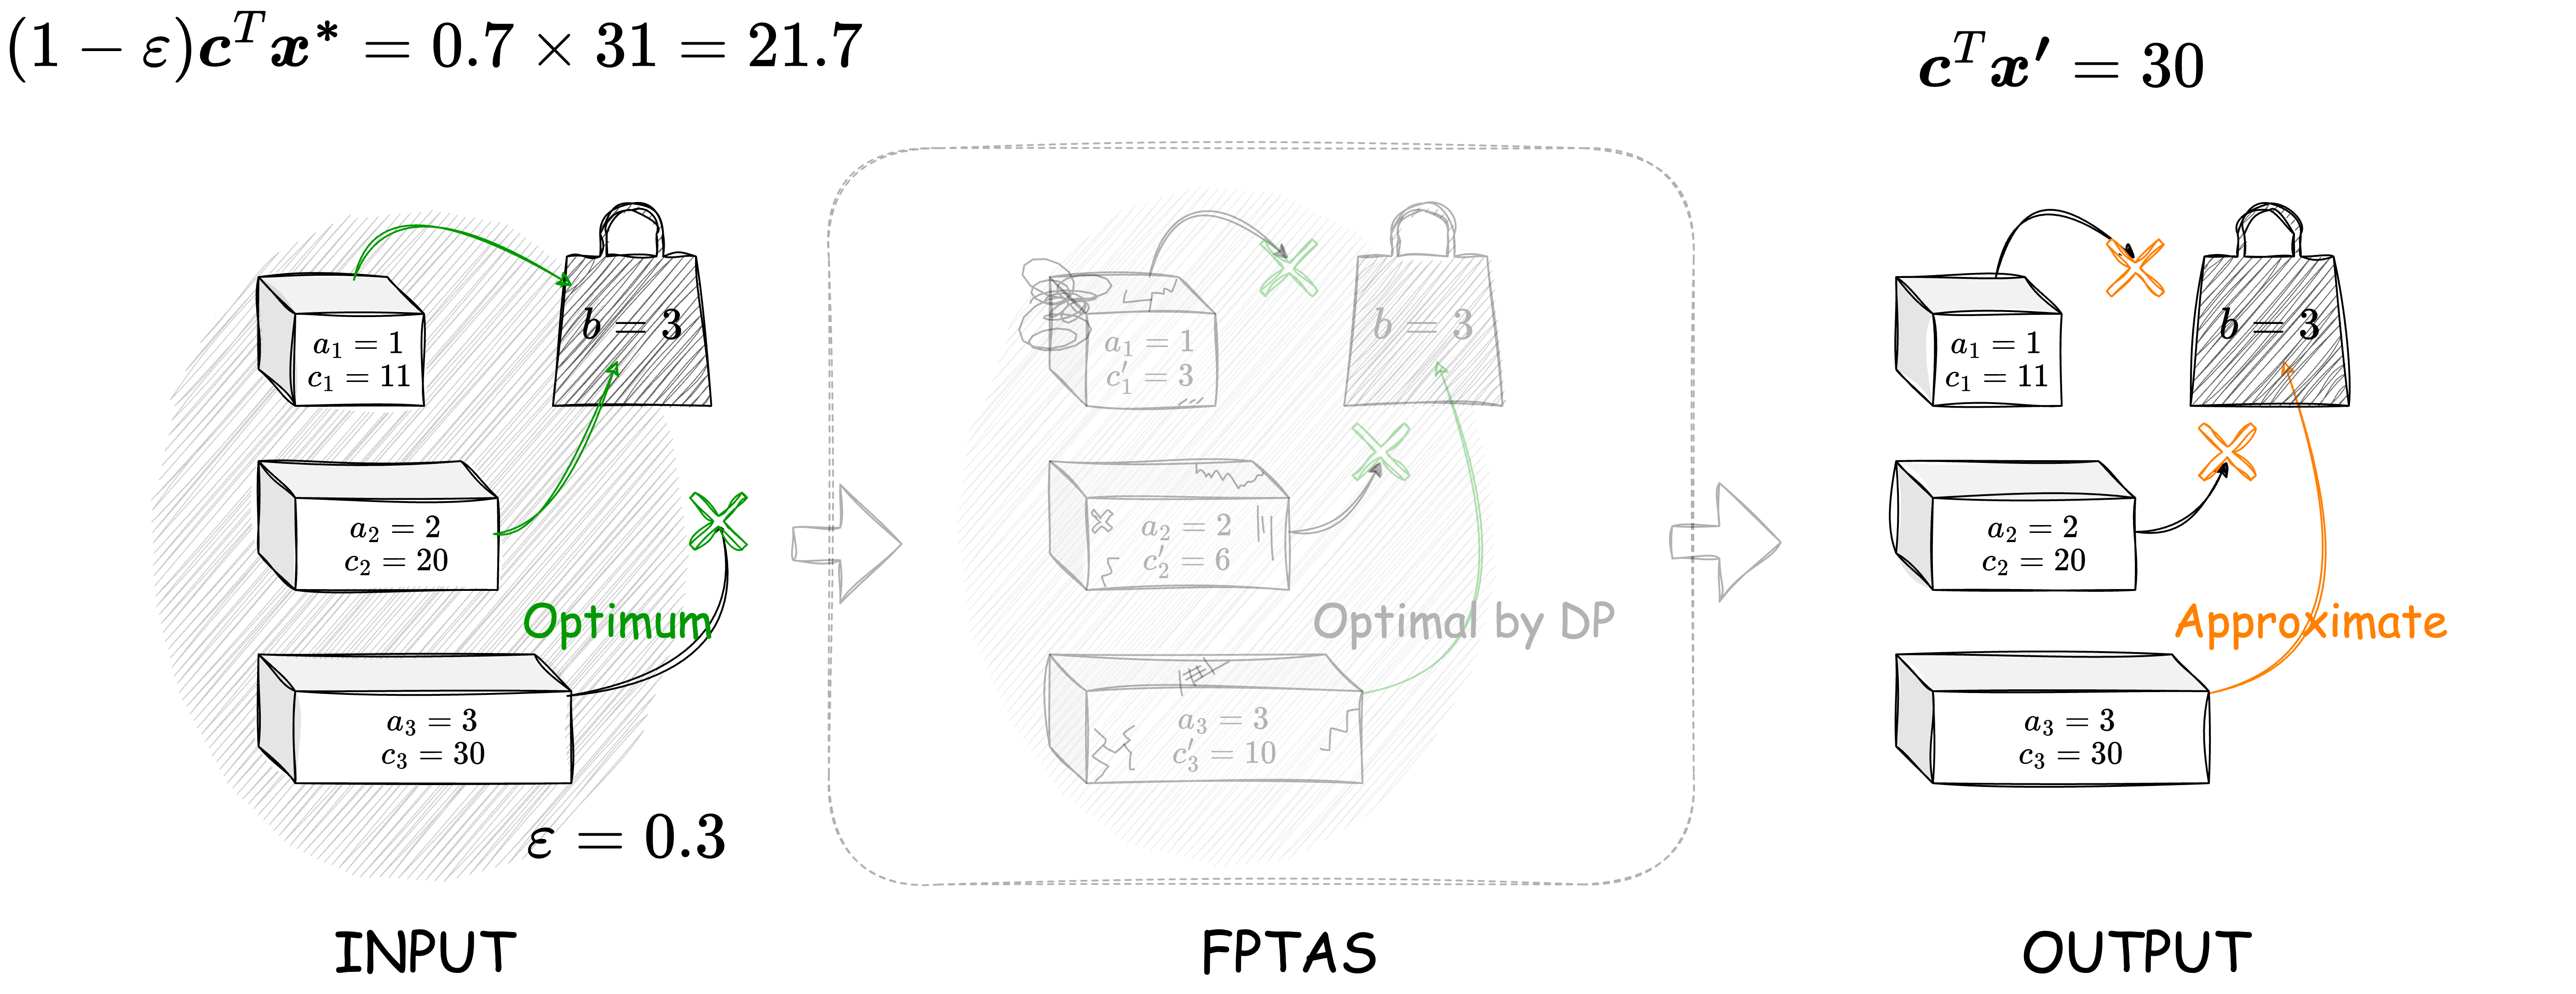
\includegraphics[width=0.8\textwidth]{figures/fptas-proof/0.png}
	\end{figure}
\end{frame}

\begin{frame}{スキームの近似保証：証明}
	\only<1>{
		\textbf{Proof.}
		\[
			\boldsymbol{c}^T \boldsymbol{x'}
			\geq K \cdot \boldsymbol{c'}^T \boldsymbol{x'}
			\geq K \cdot \boldsymbol{c'}^T \boldsymbol{x^*}
			\geq \boldsymbol{c}^T \boldsymbol{x^*} - nK
			= \boldsymbol{c}^T \boldsymbol{x^*} - \varepsilon \cdot C
			\geq (1 - \varepsilon) \cdot{\boldsymbol{c}}^T \boldsymbol{x^*}
		\]
	}

	\only<2>{
		\textbf{Proof.}
		\[
			\boldsymbol{c}^T \boldsymbol{x'}
			\geq K \cdot \boldsymbol{c'}^T \boldsymbol{x'}
			\textcolor{lightgray}{
				\geq K \cdot \boldsymbol{c'}^T \boldsymbol{x^*}
				\geq \boldsymbol{c}^T \boldsymbol{x^*} - nK
				= \boldsymbol{c}^T \boldsymbol{x^*} - \varepsilon \cdot C
				\geq (1 - \varepsilon) \cdot{\boldsymbol{c}}^T \boldsymbol{x^*}
			}
		\]
	}

	\only<3>{
		\textbf{Proof.}
		\[
			\textcolor{lightgray}{
				\boldsymbol{c}^T \boldsymbol{x'} \geq
			}
			K \cdot \boldsymbol{c'}^T \boldsymbol{x'}
			\geq K \cdot \boldsymbol{c'}^T \boldsymbol{x^*}
			\textcolor{lightgray}{
				\geq \boldsymbol{c}^T \boldsymbol{x^*} - nK
				= \boldsymbol{c}^T \boldsymbol{x^*} - \varepsilon \cdot C
				\geq (1 - \varepsilon) \cdot{\boldsymbol{c}}^T \boldsymbol{x^*}
			}
		\]
	}

	\only<4>{
		\textbf{Proof.}
		\[
			\textcolor{lightgray}{
				\boldsymbol{c}^T \boldsymbol{x'}
				\geq K \cdot \boldsymbol{c'}^T \boldsymbol{x'} \geq
			}
			K \cdot \boldsymbol{c'}^T \boldsymbol{x^*}
			\geq \boldsymbol{c}^T \boldsymbol{x^*} - nK
			\textcolor{lightgray}{
				= \boldsymbol{c}^T \boldsymbol{x^*} - \varepsilon \cdot C
				\geq (1 - \varepsilon) \cdot{\boldsymbol{c}}^T \boldsymbol{x^*}
			}
		\]
	}

	\only<5>{
		\textbf{Proof.}
		\[
			\textcolor{lightgray}{
				\boldsymbol{c}^T \boldsymbol{x'}
				\geq K \cdot \boldsymbol{c'}^T \boldsymbol{x'}
				\geq K \cdot \boldsymbol{c'}^T \boldsymbol{x^*} \geq
			}
			\boldsymbol{c}^T \boldsymbol{x^*} - nK
			= \boldsymbol{c}^T \boldsymbol{x^*} - \varepsilon \cdot C
			\textcolor{lightgray}{
				\geq (1 - \varepsilon) \cdot{\boldsymbol{c}}^T \boldsymbol{x^*}
			}
		\]
	}

	\only<6>{
		\textbf{Proof.}
		\[
			\textcolor{lightgray}{
				\boldsymbol{c}^T \boldsymbol{x'}
				\geq K \cdot \boldsymbol{c'}^T \boldsymbol{x'}
				\geq K \cdot \boldsymbol{c'}^T \boldsymbol{x^*}
				\geq \boldsymbol{c}^T \boldsymbol{x^*} - nK =
			}
			\boldsymbol{c}^T \boldsymbol{x^*} - \varepsilon \cdot C
			\geq (1 - \varepsilon) \cdot{\boldsymbol{c}}^T \boldsymbol{x^*}
		\]
		\qed
	}

	\begin{columns}
		\begin{column}{0.65\columnwidth}
			\only<2>{
				\begin{itemize}
					\item \alert{\(c'_i = \lfloor c_i / K \rfloor \le c_i / K\)} より成り立つ
				\end{itemize}
				\begin{figure}
					\centering
					
\includegraphics[width=1.0\textwidth]{figures/fptas-proof/1.png}
				\end{figure}
			}

			\only<3>{
				\begin{itemize}
					\item \(\boldsymbol{x'}\) は \(\boldsymbol{c'}\) に対する最適解
				\end{itemize}
				\begin{figure}
					\centering
					
\includegraphics[width=1.0\textwidth]{figures/fptas-proof/2.png}
				\end{figure}
			}

			\only<4>{
				\begin{itemize}
					\item \(c_i / K - 1 \le \lfloor c_i / K \rfloor = c'_i\) より \(Kc'_i \ge c_i - K\)
					\item	\(\alert{K \cdot \boldsymbol{c'}^T \boldsymbol{x^*}} \geq (\boldsymbol{c} - (K)_n)^T \boldsymbol{x^*} \geq \alert{\boldsymbol{c}^T \boldsymbol{x^*} - nK}\)
				\end{itemize}

				\begin{figure}
					\centering
					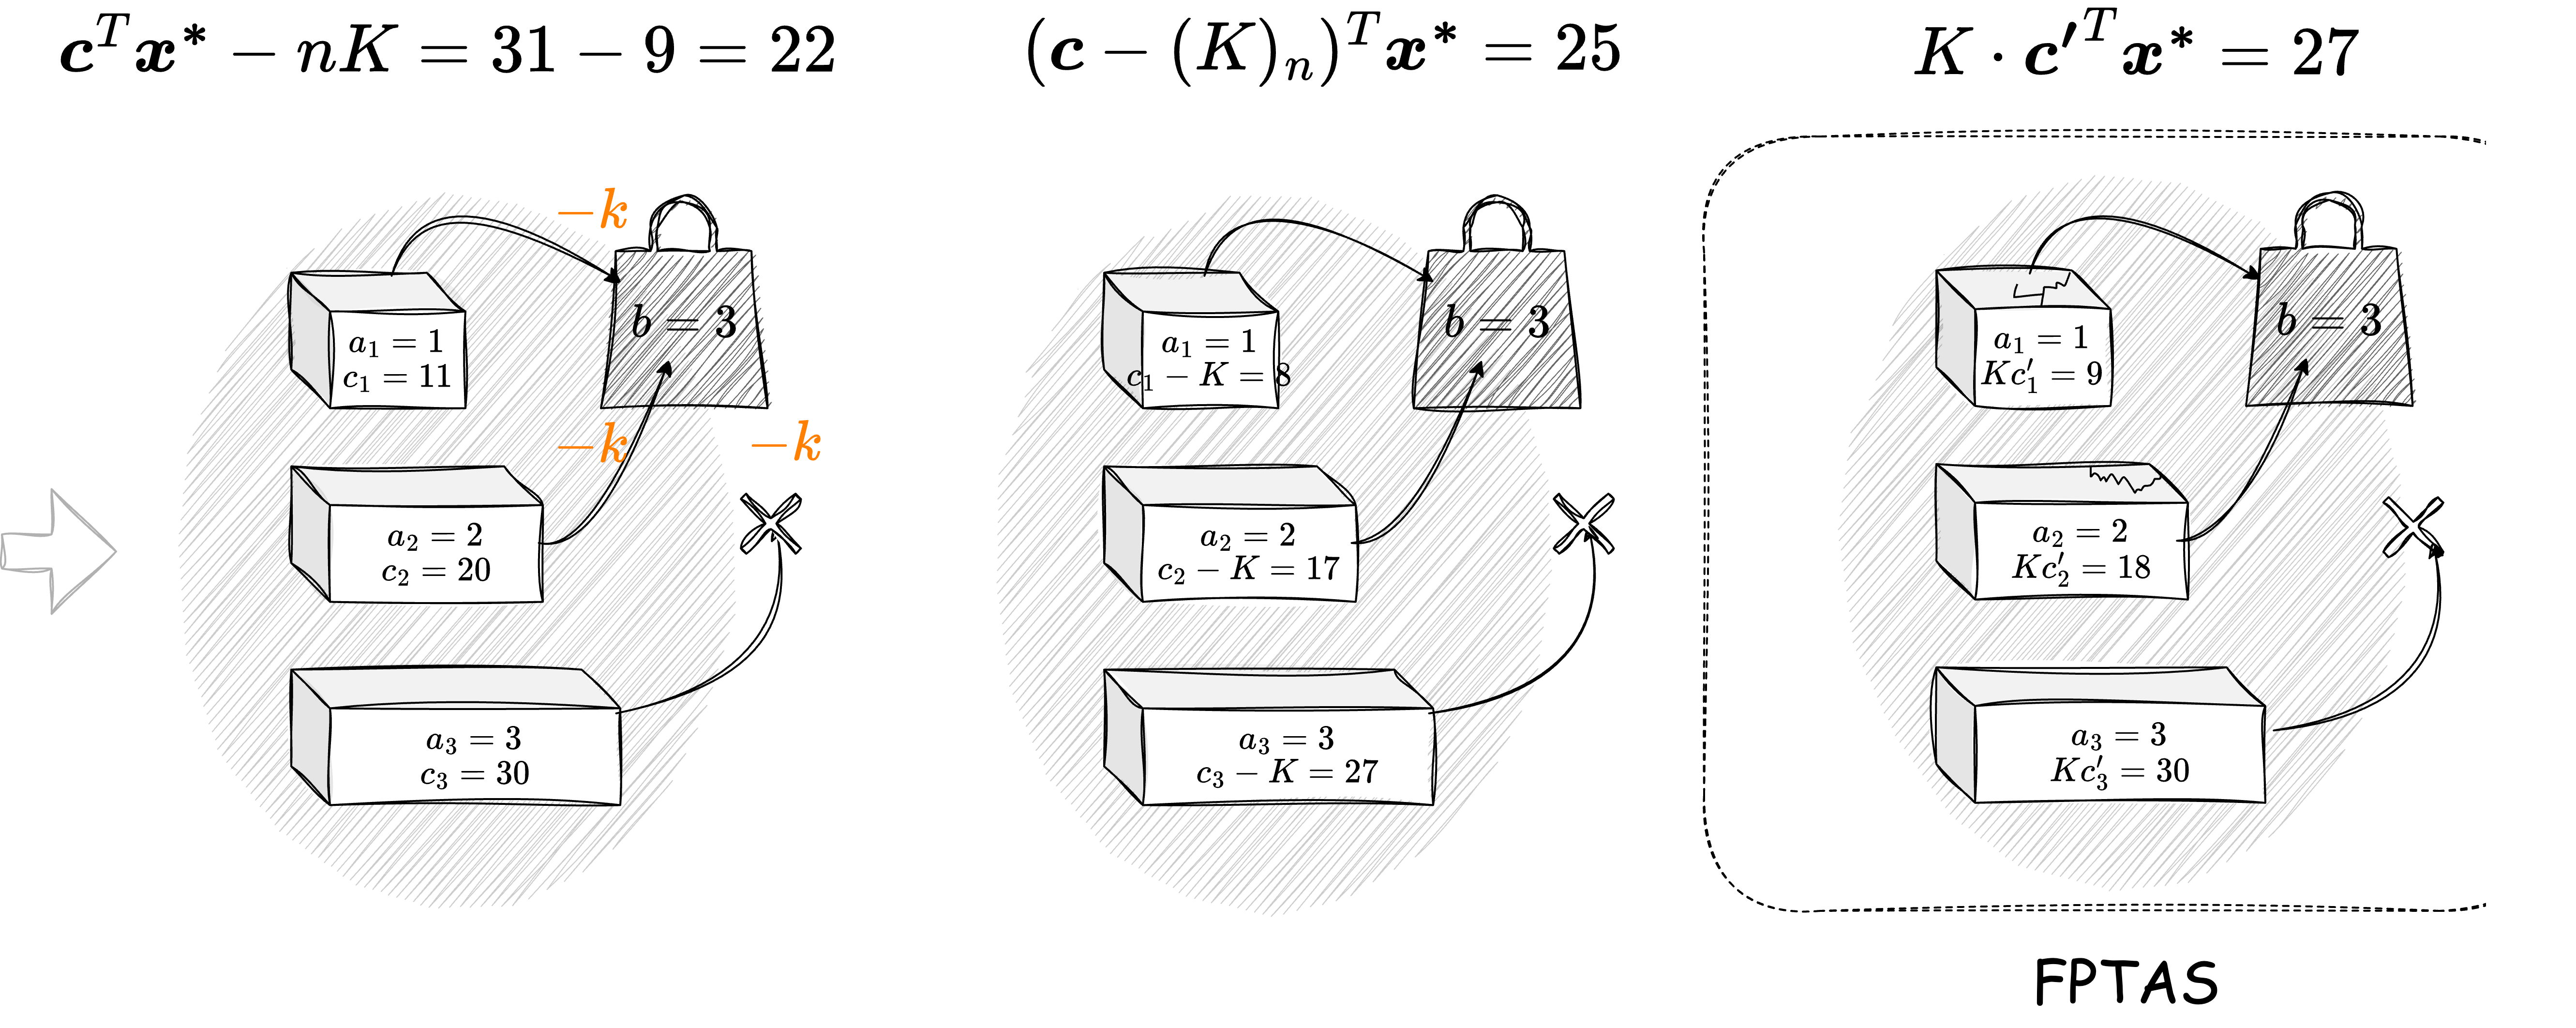
\includegraphics[width=0.95\textwidth]{figures/fptas-proof/3.png}
				\end{figure}
			}

			\only<5>{
				\begin{itemize}
					\item \(K\) の定義から，\(nK = n\cdot \varepsilon C/n = \varepsilon C\)
				\end{itemize}

				\begin{figure}
					\centering
					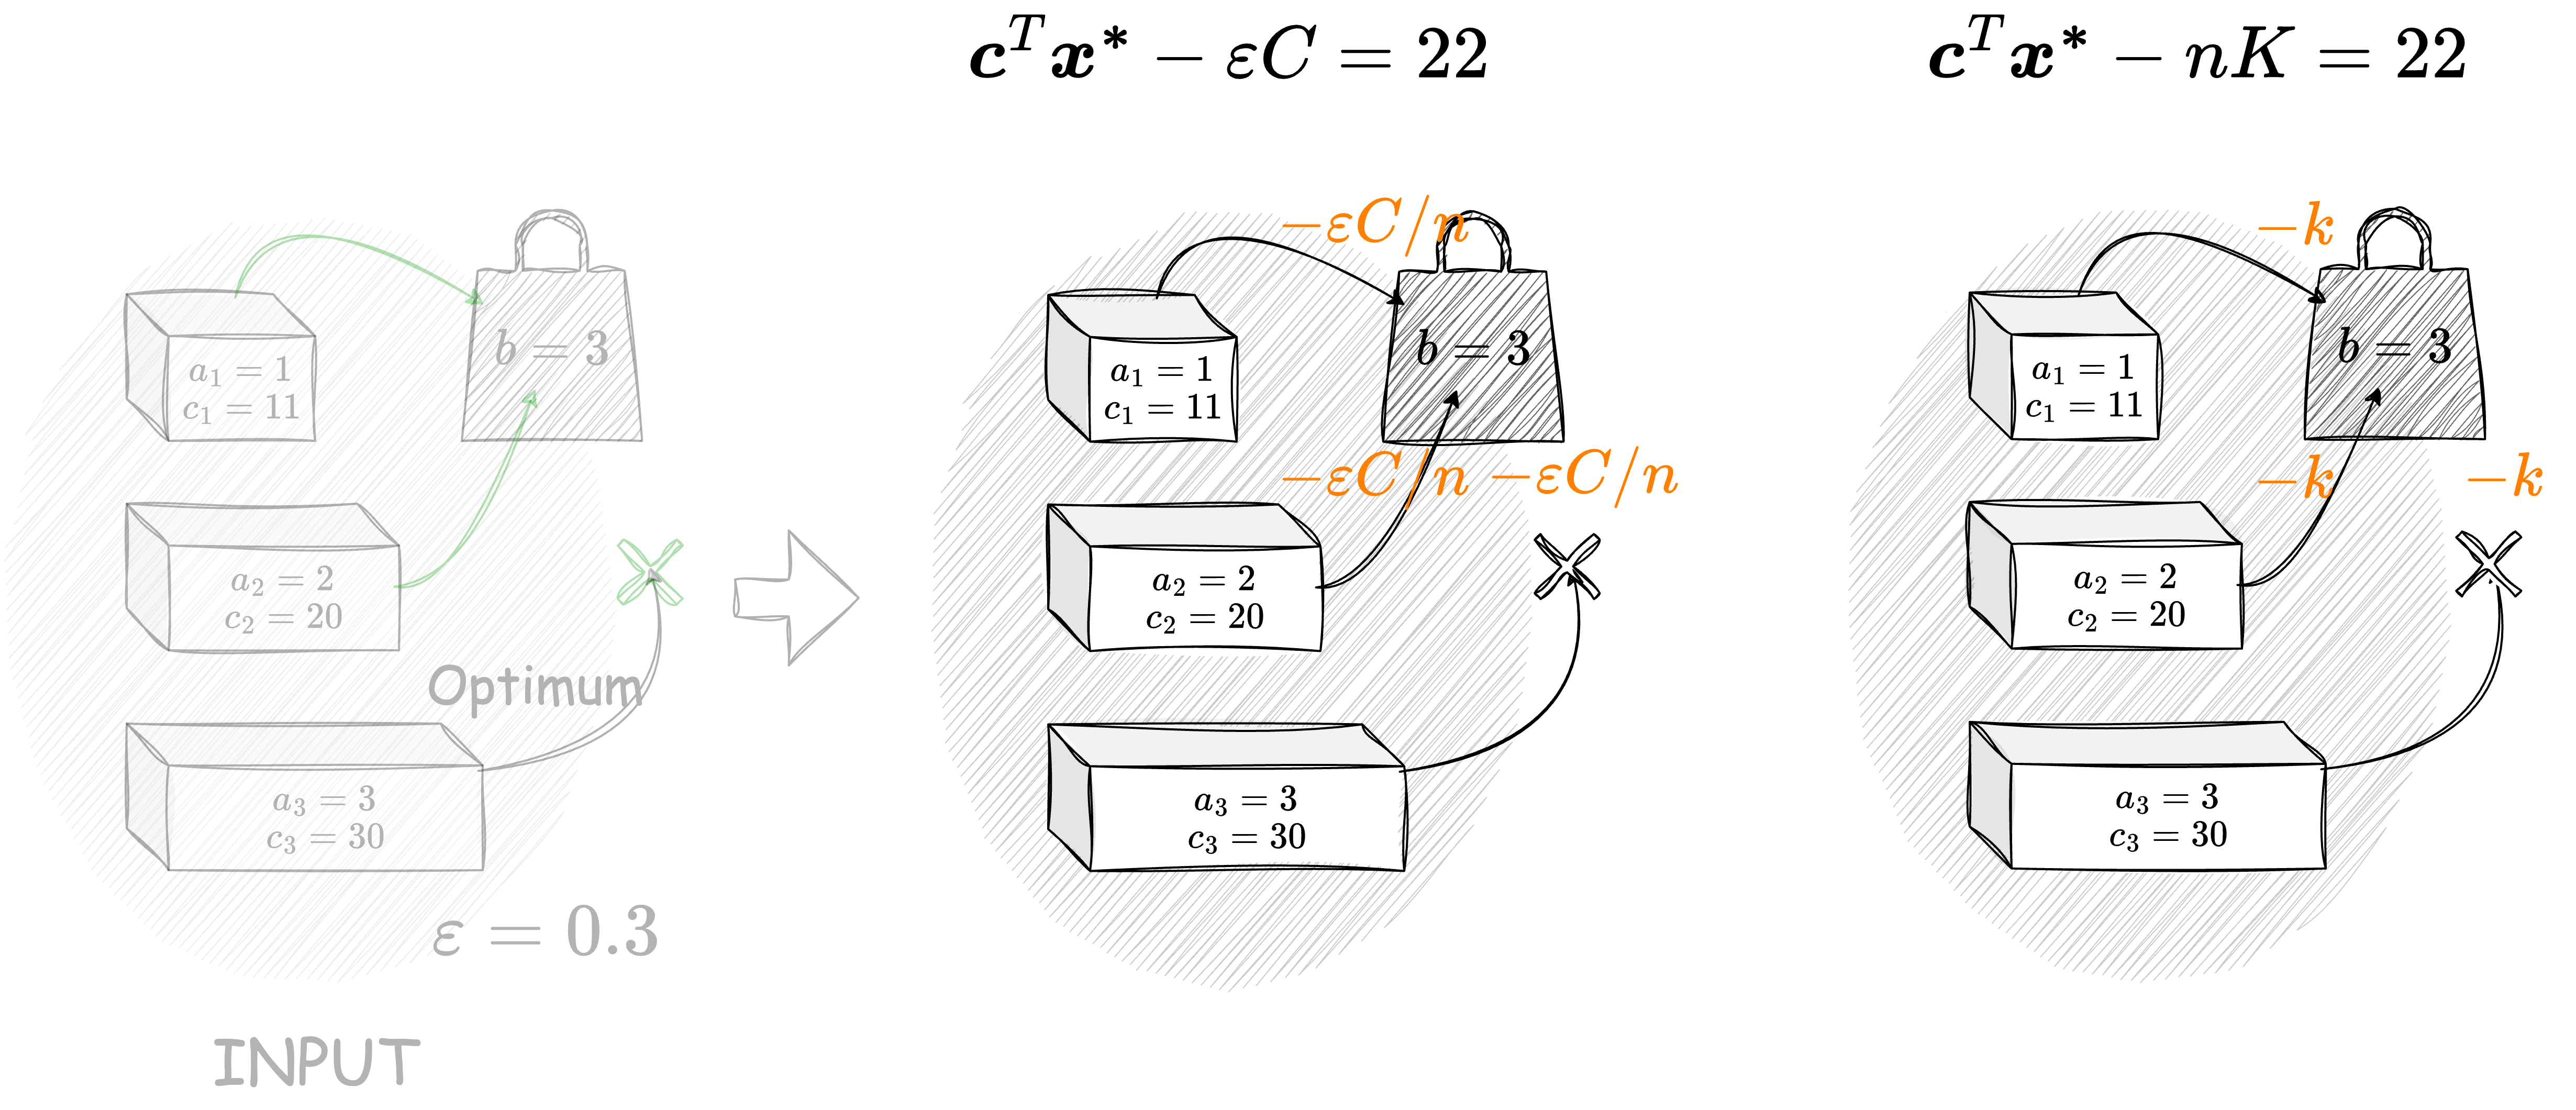
\includegraphics[width=1.0\textwidth]{figures/fptas-proof/4.png}
				\end{figure}
			}

			\only<6>{
				\begin{itemize}
					\item 元の問題の最適値 \(\boldsymbol{c}^T\boldsymbol{x^*}\) は，商品の最高価値 \(C\) 以上であるはず\footnote{すべての商品の重みはナップサックの容量以下であることを仮定}
				\end{itemize}

				\begin{figure}
					\centering
					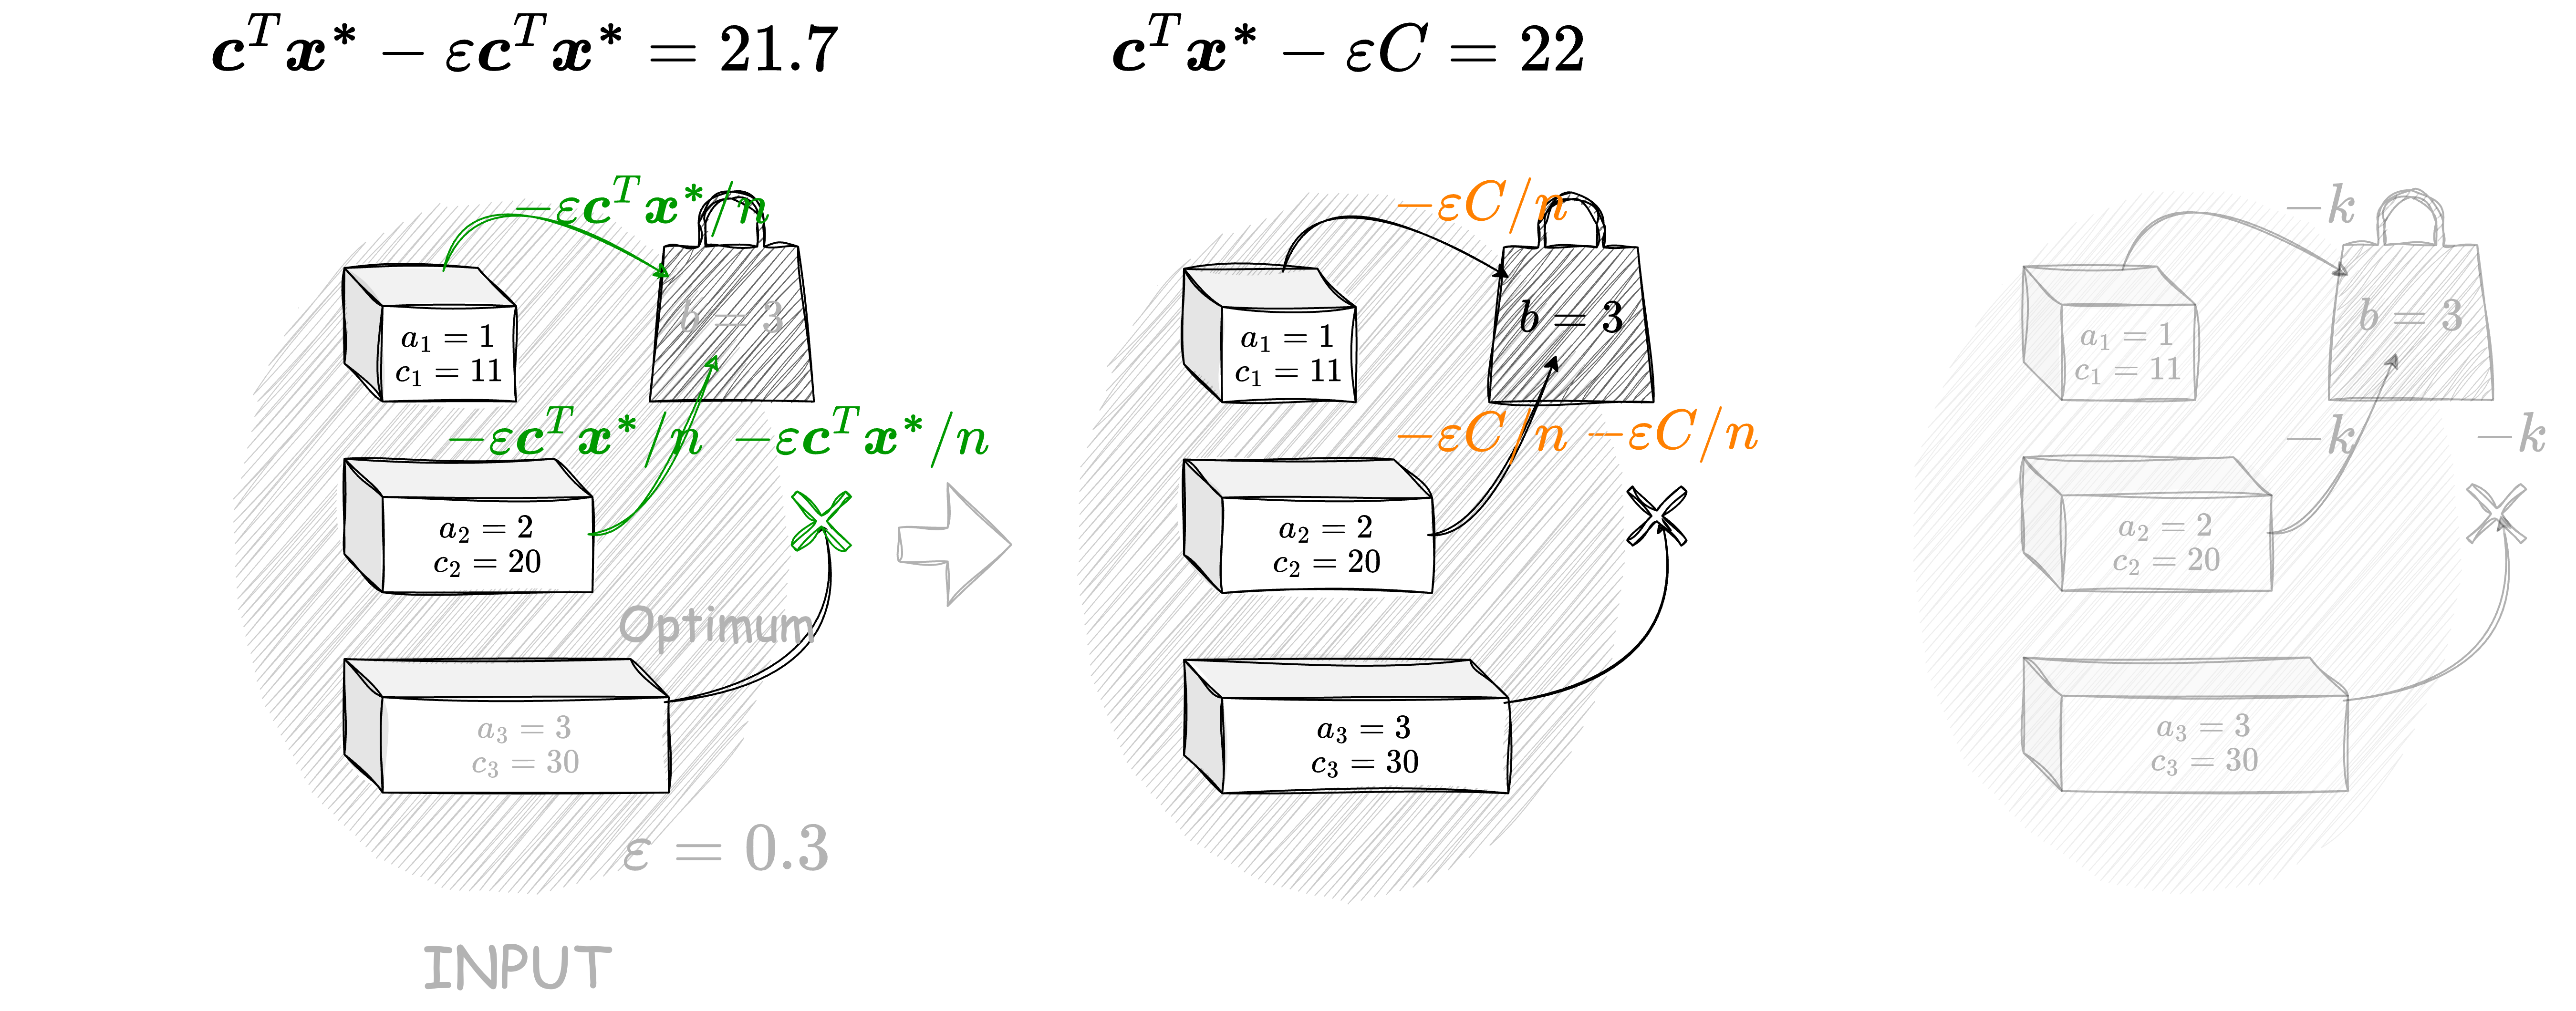
\includegraphics[width=0.95\textwidth]{figures/fptas-proof/5.png}
				\end{figure}
			}
		\end{column}

		\begin{column}{0.35\columnwidth}
			\vskip 0.5em
			\begin{block}{Notations}
				\begin{itemize}
					\leftskip 1.0em
					\item[\(\boldsymbol{c}\): ] 価値ベクトル
					\item[\(C\): ] 価値の最大値
					\item[\(K\): ] スケーラー \(\varepsilon C / n\)
					\item[\(\boldsymbol{c'}\): ] スケールダウン後の \\ 価値ベクトル \(\lfloor \boldsymbol{c} / K \rfloor\)
					\item[\(\boldsymbol{x^*}\): ] 最適解
					\item[\(\boldsymbol{x'}\): ] スキームの解
				\end{itemize}
			\end{block}
		\end{column}
	\end{columns}
\end{frame}

\begin{frame}{スキームの計算時間}
	\begin{lemma}[スキームの計算時間]
		スキームは，\alert{\(\mathcal{O}(n^3 / \varepsilon)\)} 時間で動作する．
	\end{lemma}

	\textbf{Proof.}
	\begin{itemize}
		\item アイテムの価値をスケールダウン\footnote{\(K = \varepsilon C / n, c'_i = \lfloor c_i / K\rfloor \le \lfloor n / \varepsilon \rfloor\)}するのに \(\mathcal{O}(n)\) 時間
		\item 動的計画法の計算時間は，\(\mathcal{O}(n^2 \max_i\{c'_i\}) = \mathcal{O}(n^3 / \varepsilon)\) \qed
	\end{itemize}
\end{frame}

\begin{frame}{まとめ}
	\begin{theorem*}[restaed: \alert{ナップサック問題の FPTAS}]
		ナップサック問題に対して，任意の正数 \(\varepsilon < 1\) に対し，\alert{\(\mathcal{O}(n^3/\varepsilon)\)} 時間で \alert{\((1 - \varepsilon)\)} 倍の近似解を求めるスキームが存在する．
	\end{theorem*}
\end{frame}

\begin{frame}[standout]
	Any Questions?
\end{frame}

\appendix{}

\begin{frame}{ナップサックの容量に基づく擬多項式時間アルゴリズム}
	\begin{theorem}[ナップサックの容量に基づく擬多項式時間アルゴリズム]
		ナップサック問題に対して，\alert{\(\mathcal{O}(nb)\) 時間}で\alert{最適解}を求めるアルゴリズムが存在する．
	\end{theorem}

	\begin{algorithm}[容量に基づく動的計画法]
		\begin{itemize}
			\item \(dp[i][j] := \) 商品 \(i\) までの中から，容量 \(j\) 以下で選んだときの価値の最大値
			\item \(dp[0][:] = 0\)
			\item \(
			      dp[i][j] =
			      \begin{cases}
				      dp[i-1][j]                              & \textit{if } j - a_i < 0 \textit{,} \\
				      \max(dp[i-1][j],\ dp[i-1][j-a_i] + c_i) & \textit{otherwise.}
			      \end{cases}
			      \)
			\item \(dp[n][b]\) を出力する
		\end{itemize}
	\end{algorithm}
\end{frame}

\begin{frame}{容量に基づく動的計画法：動作例（\(i\) 番目のアイテムを選択するとき）}
	\begin{figure}
		\centering
		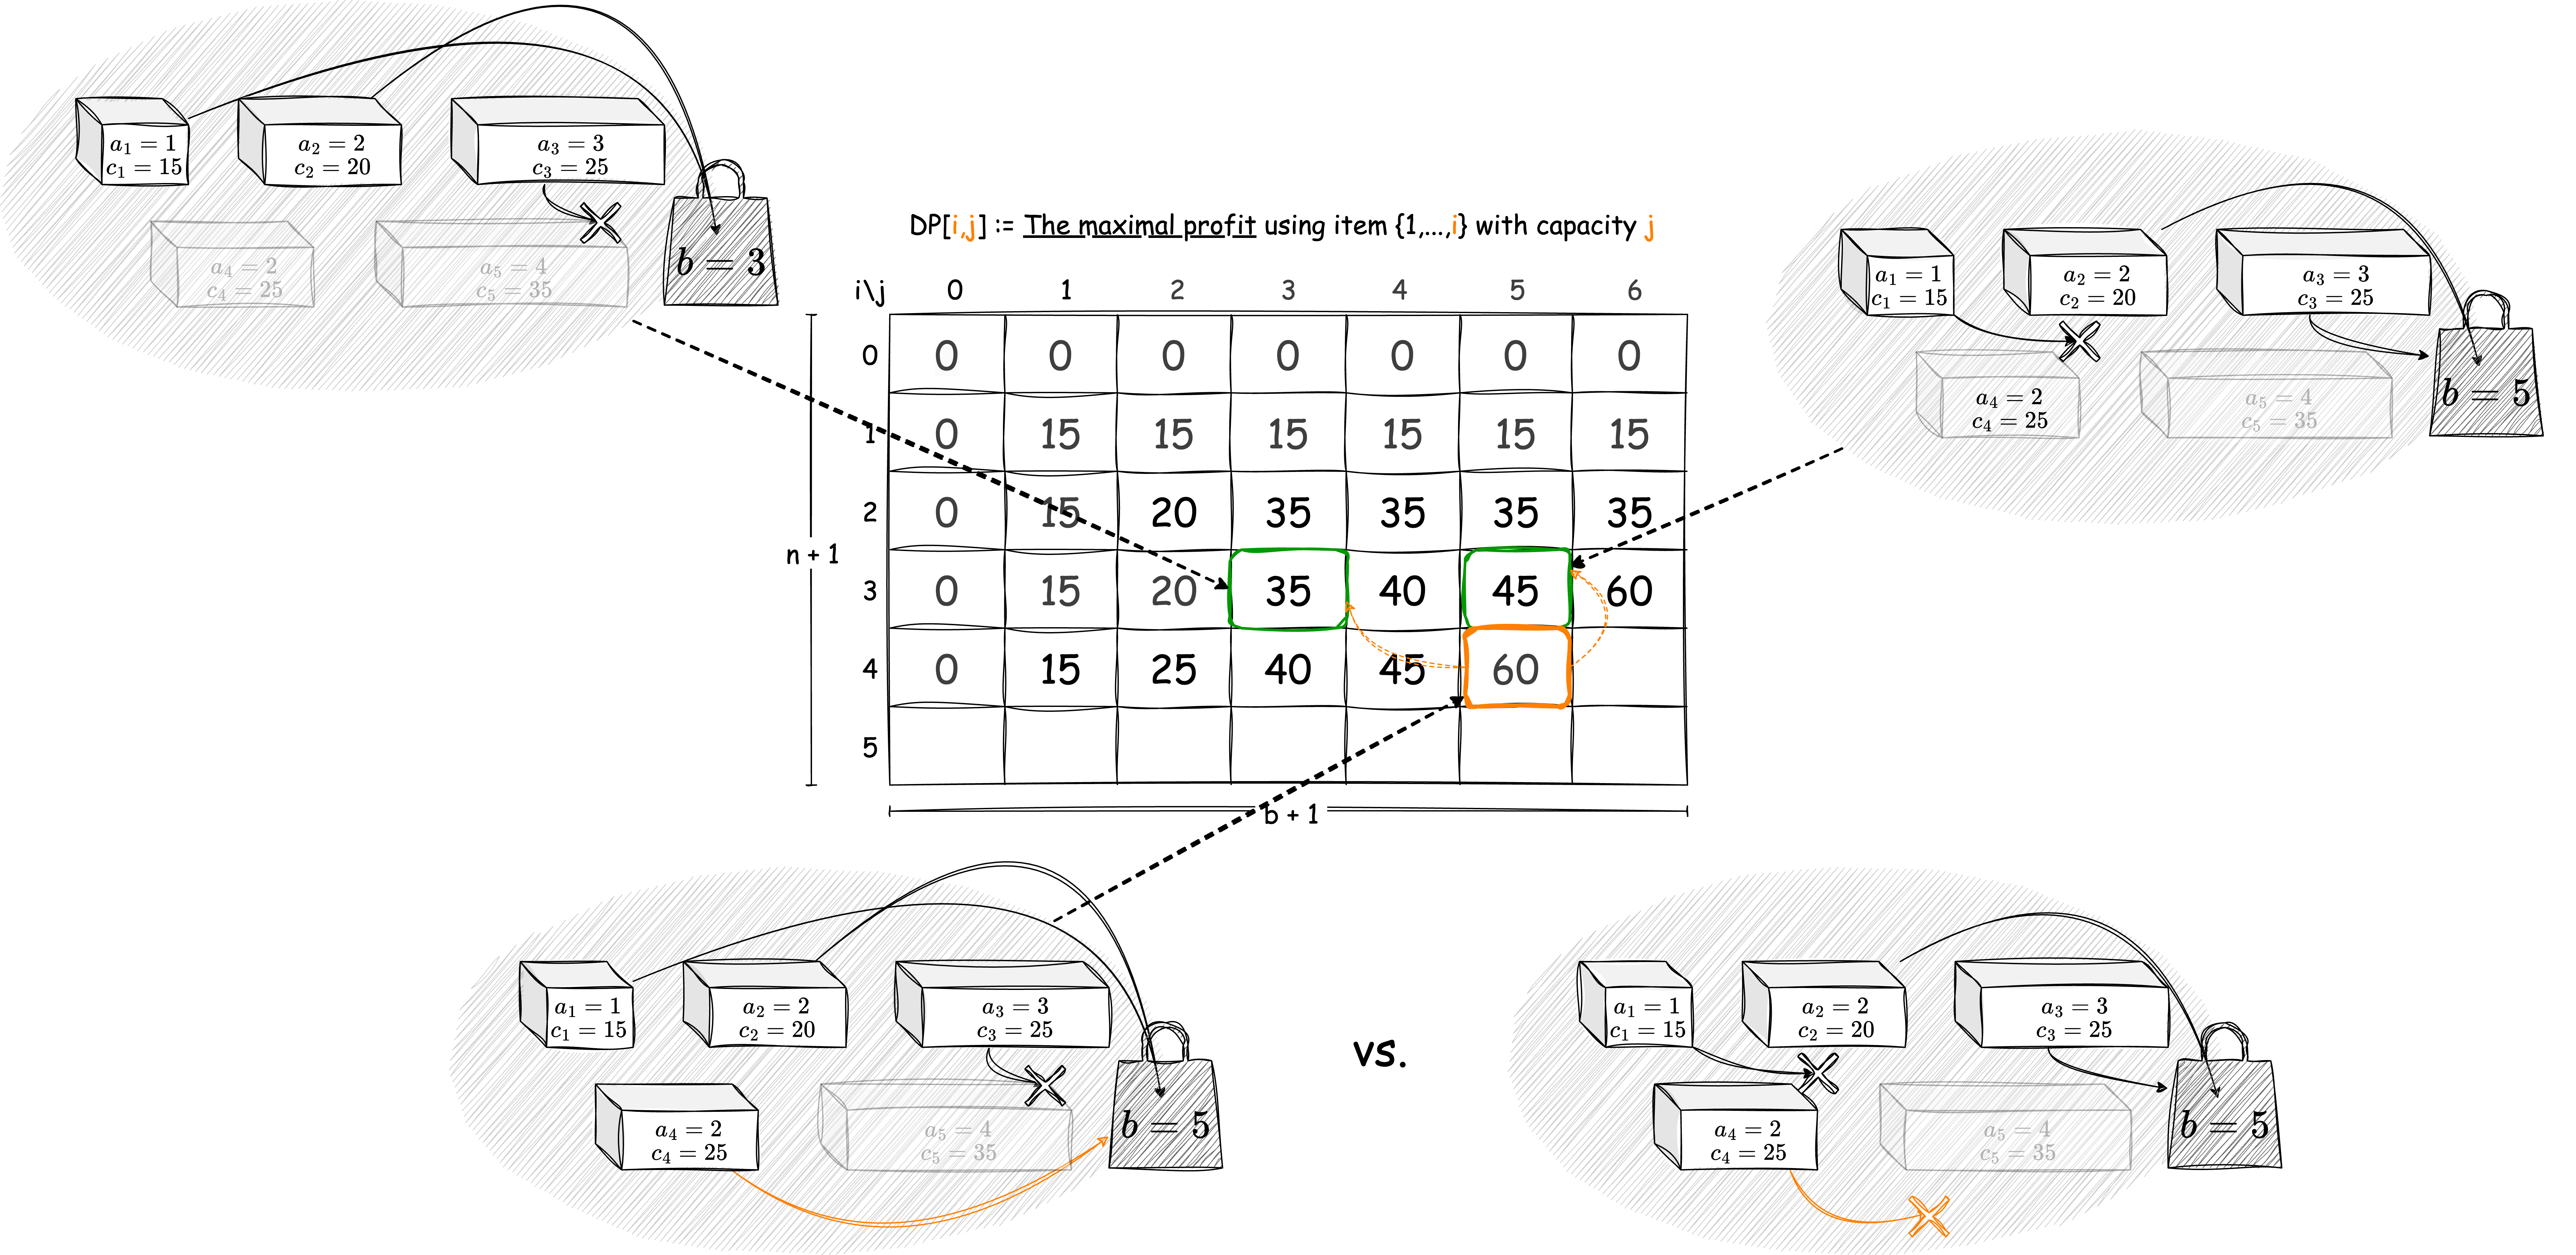
\includegraphics[width=1.0\textwidth]{figures/dp/1.png}
	\end{figure}
\end{frame}

\begin{frame}{容量に基づく動的計画法：動作例（\(i\) 番目のアイテムを選択しないとき）}
	\begin{figure}
		\centering
		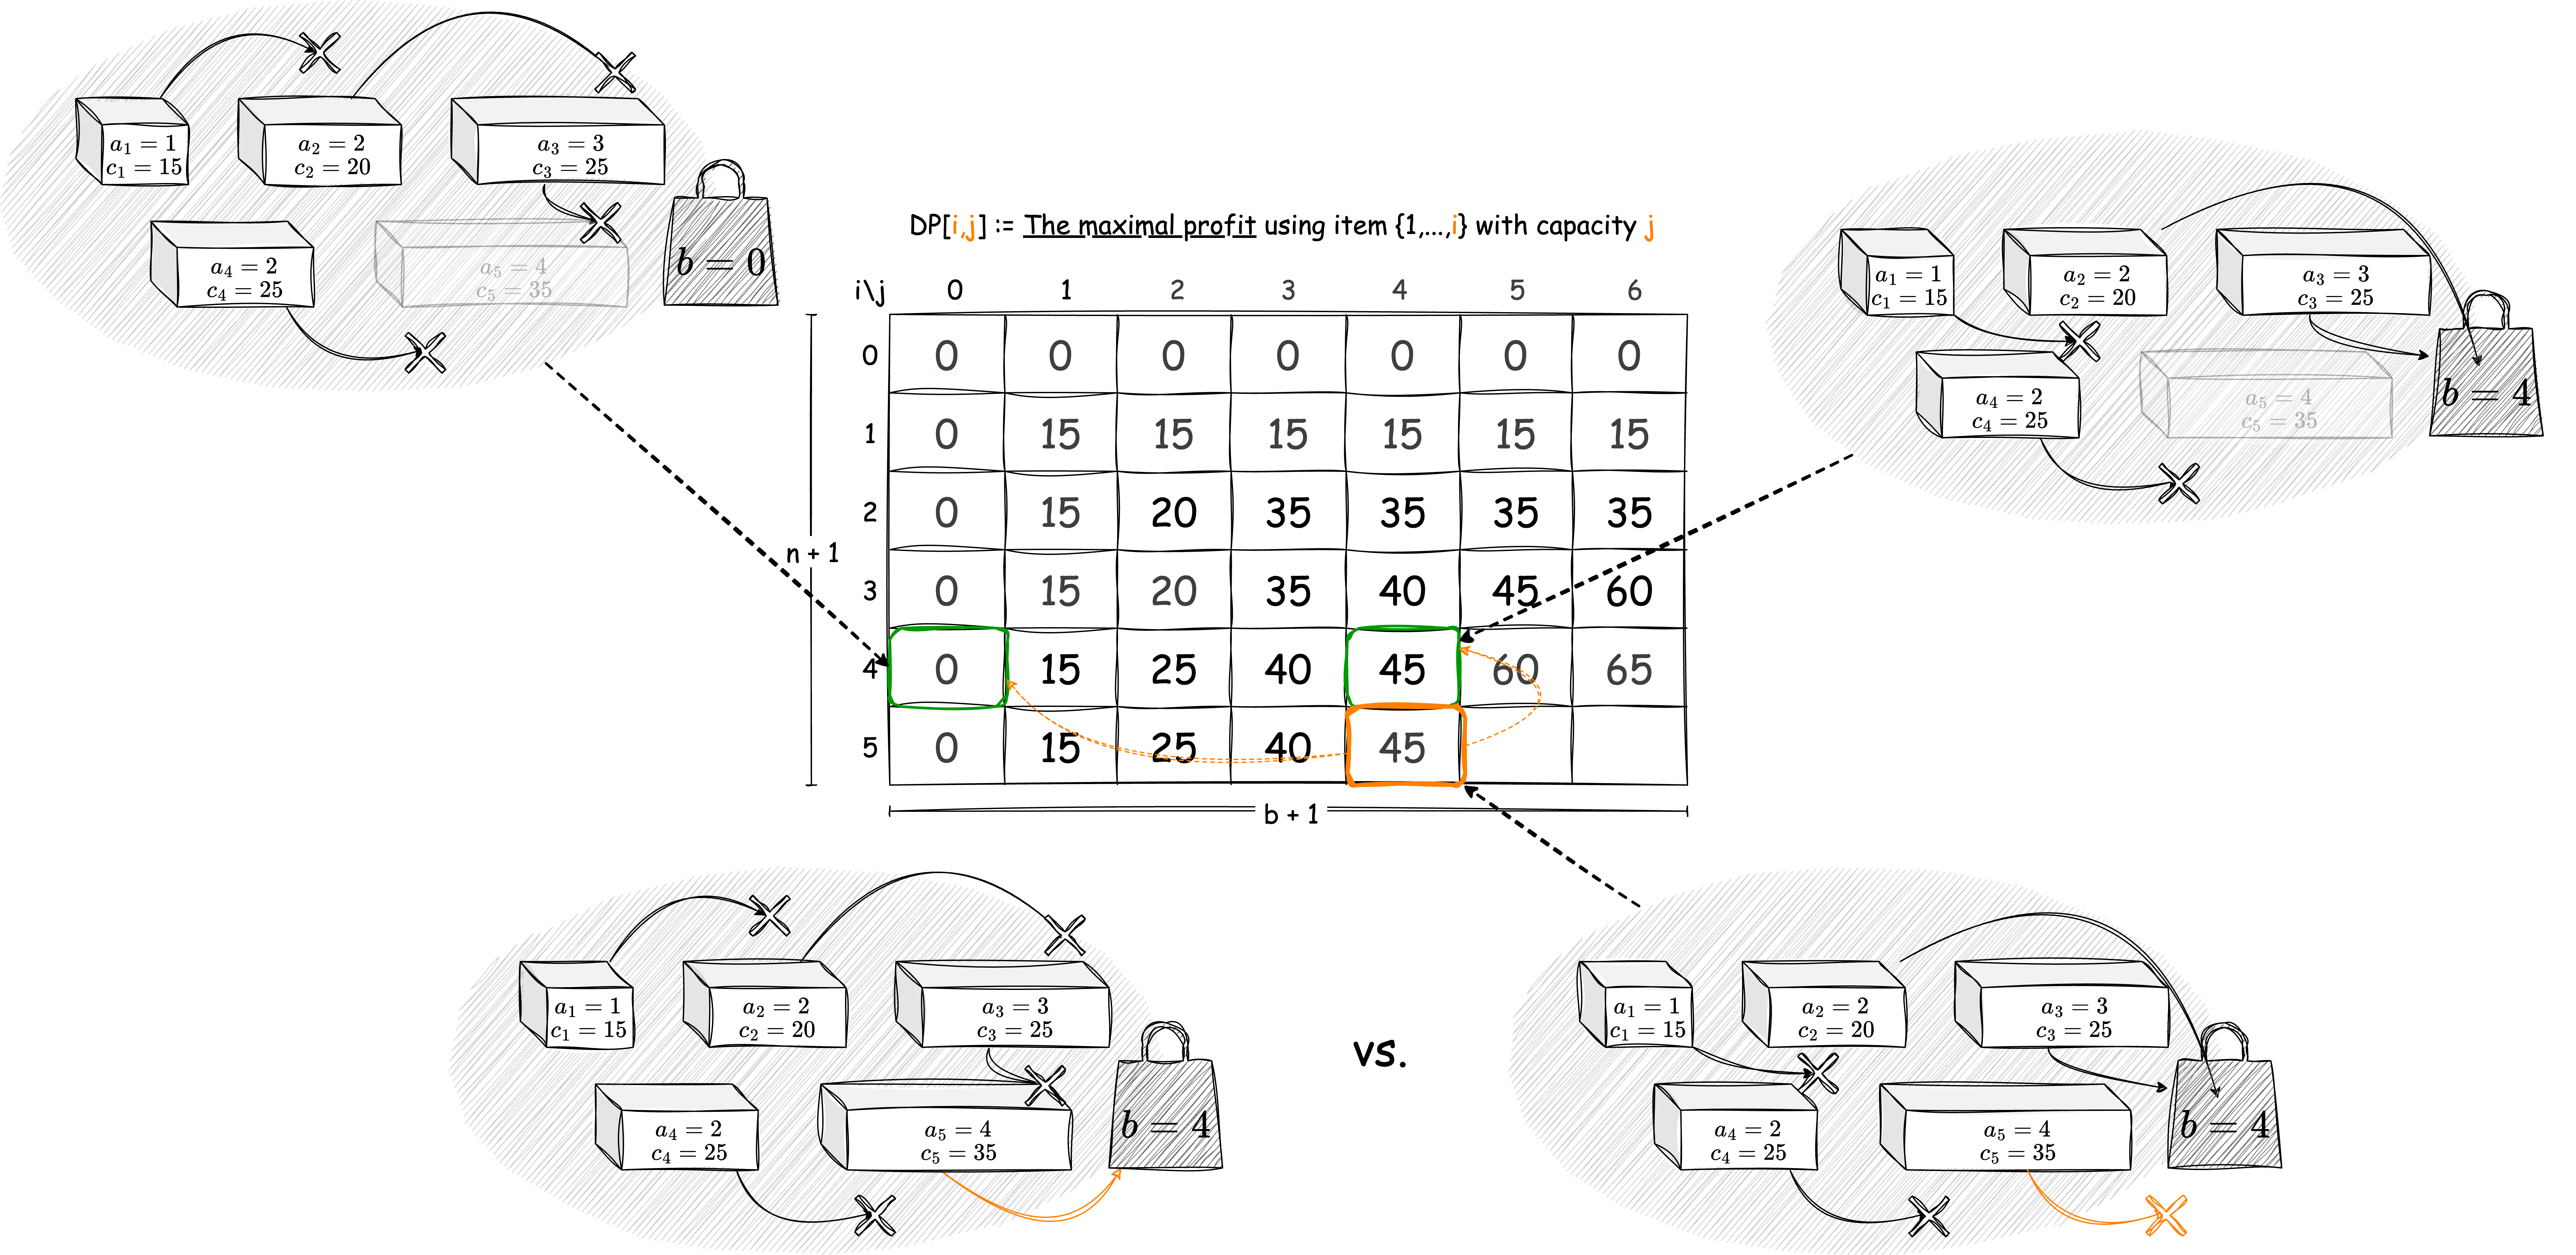
\includegraphics[width=1.0\textwidth]{figures/dp/2.png}
	\end{figure}
\end{frame}

\begin{frame}{FPTAS 再び？}

	\begin{conjecture}[\alert{重みをスケールダウンさせる FPTAS}]
		ナップサック問題に対して，任意の正数 \(\varepsilon < 1\) に対し，\alert{\(\mathcal{O}(n^3/\varepsilon)\)} 時間で \alert{\((1 - \varepsilon)\)} 倍の近似解を求める重みをスケールダウンするようなスキームが存在する？？？
	\end{conjecture}

	\begin{scheme}[重みをスケールダウンさせるスキーム]
		\begin{itemize}
			\item 与えられた \(0 < \varepsilon < 1\) に対し，\alert{\(K = \varepsilon b / n\)} を定める
			\item 重みを \alert{\(a_i' = \lceil a_i / K \rceil\)} で修正する%
			      \footnote{このとき，\(a'_i = \lceil n / \epsilon \cdot a_i / b\rceil \le \lceil n / \epsilon \rceil \) となる．}
			\item 修正重みとナップサックの容量 \alert{\(\lfloor b / K \rfloor\)} のもとで，動的計画法を適用する%
			      \footnote{このとき \(\boldsymbol{a'}^T\boldsymbol{x} \le \lfloor b / K\rfloor\) となる \(\boldsymbol{x}\) に対して，\(\boldsymbol{a}^T\boldsymbol{x} \le K \boldsymbol{a'}^T\boldsymbol{x} \le b\) を満たすことに注意する．}
		\end{itemize}
	\end{scheme}
\end{frame}

\begin{frame}{重みをスケールダウンさせるスキームの近似保証}
	\vskip 1em

	\begin{conjecture}[重みをスケールダウンさせるスキームの近似保証]
		重みをスケールダウンさせるスキームが出力する解 \(\boldsymbol{x'}\) は，次式を満たす？？？
		\[
			\alert{\boldsymbol{c}^T \boldsymbol{x'} \geq (1 - \varepsilon) \cdot{\boldsymbol{c}}^T \boldsymbol{x^*}}
		\]
	\end{conjecture}

	\textbf{Idea of Proof?}
	\begin{itemize}
		\item スケーリングの誤差によって，近似解では高々 \(nK = \varepsilon b\) の空き容量が生じる
		\item 最適解と近似解における価値あたりの重みを導入する
		      \[
			      \boldsymbol{c}^T \boldsymbol{x^*} / \boldsymbol{a}^T \boldsymbol{x^*}, \quad
			      \boldsymbol{c}^T \boldsymbol{x'} / \boldsymbol{a'}^T \boldsymbol{x'}
		      \]
		\item \(\boldsymbol{c}^T\boldsymbol{x'} \le \boldsymbol{c}^T\boldsymbol{x^*}\)
		\item \(K a'_i \ge a_i\) より，\(\boldsymbol{a'}^T\boldsymbol{x} \ge K \boldsymbol{a}^T\boldsymbol{x}\) と \(c_i / a_i \le c_i / K a'_i\) が成り立つ
	\end{itemize}
\end{frame}

\begin{frame}{\(\mathcal{NP}\)-hardness}
	\begin{theorem}
		ナップサック問題は \(\mathcal{NP}\)-hard である．
	\end{theorem}

	\begin{problem}[分割問題]
	\begin{itemize}
		\leftskip 3em
		\item[Input: ] \(\boldsymbol{a} \in \mathbb{Z}^n_{+}\)
		\item[Output: ] \(\boldsymbol{x} \in \{0, 1\}^n\) such that
		      \[
			      \alert{\boldsymbol{x}^T \boldsymbol{a} = \frac{1}{2} \sum_{i=1}^n a_i}
		      \]
	\end{itemize}
	\end{problem}

	\begin{theorem}
		分割問題は \(\mathcal{NP}\)-hard である．
	\end{theorem}
\end{frame}

\begin{frame}{分割問題からナップサック問題への多項式時間帰着}
	\begin{figure}
		\centering
		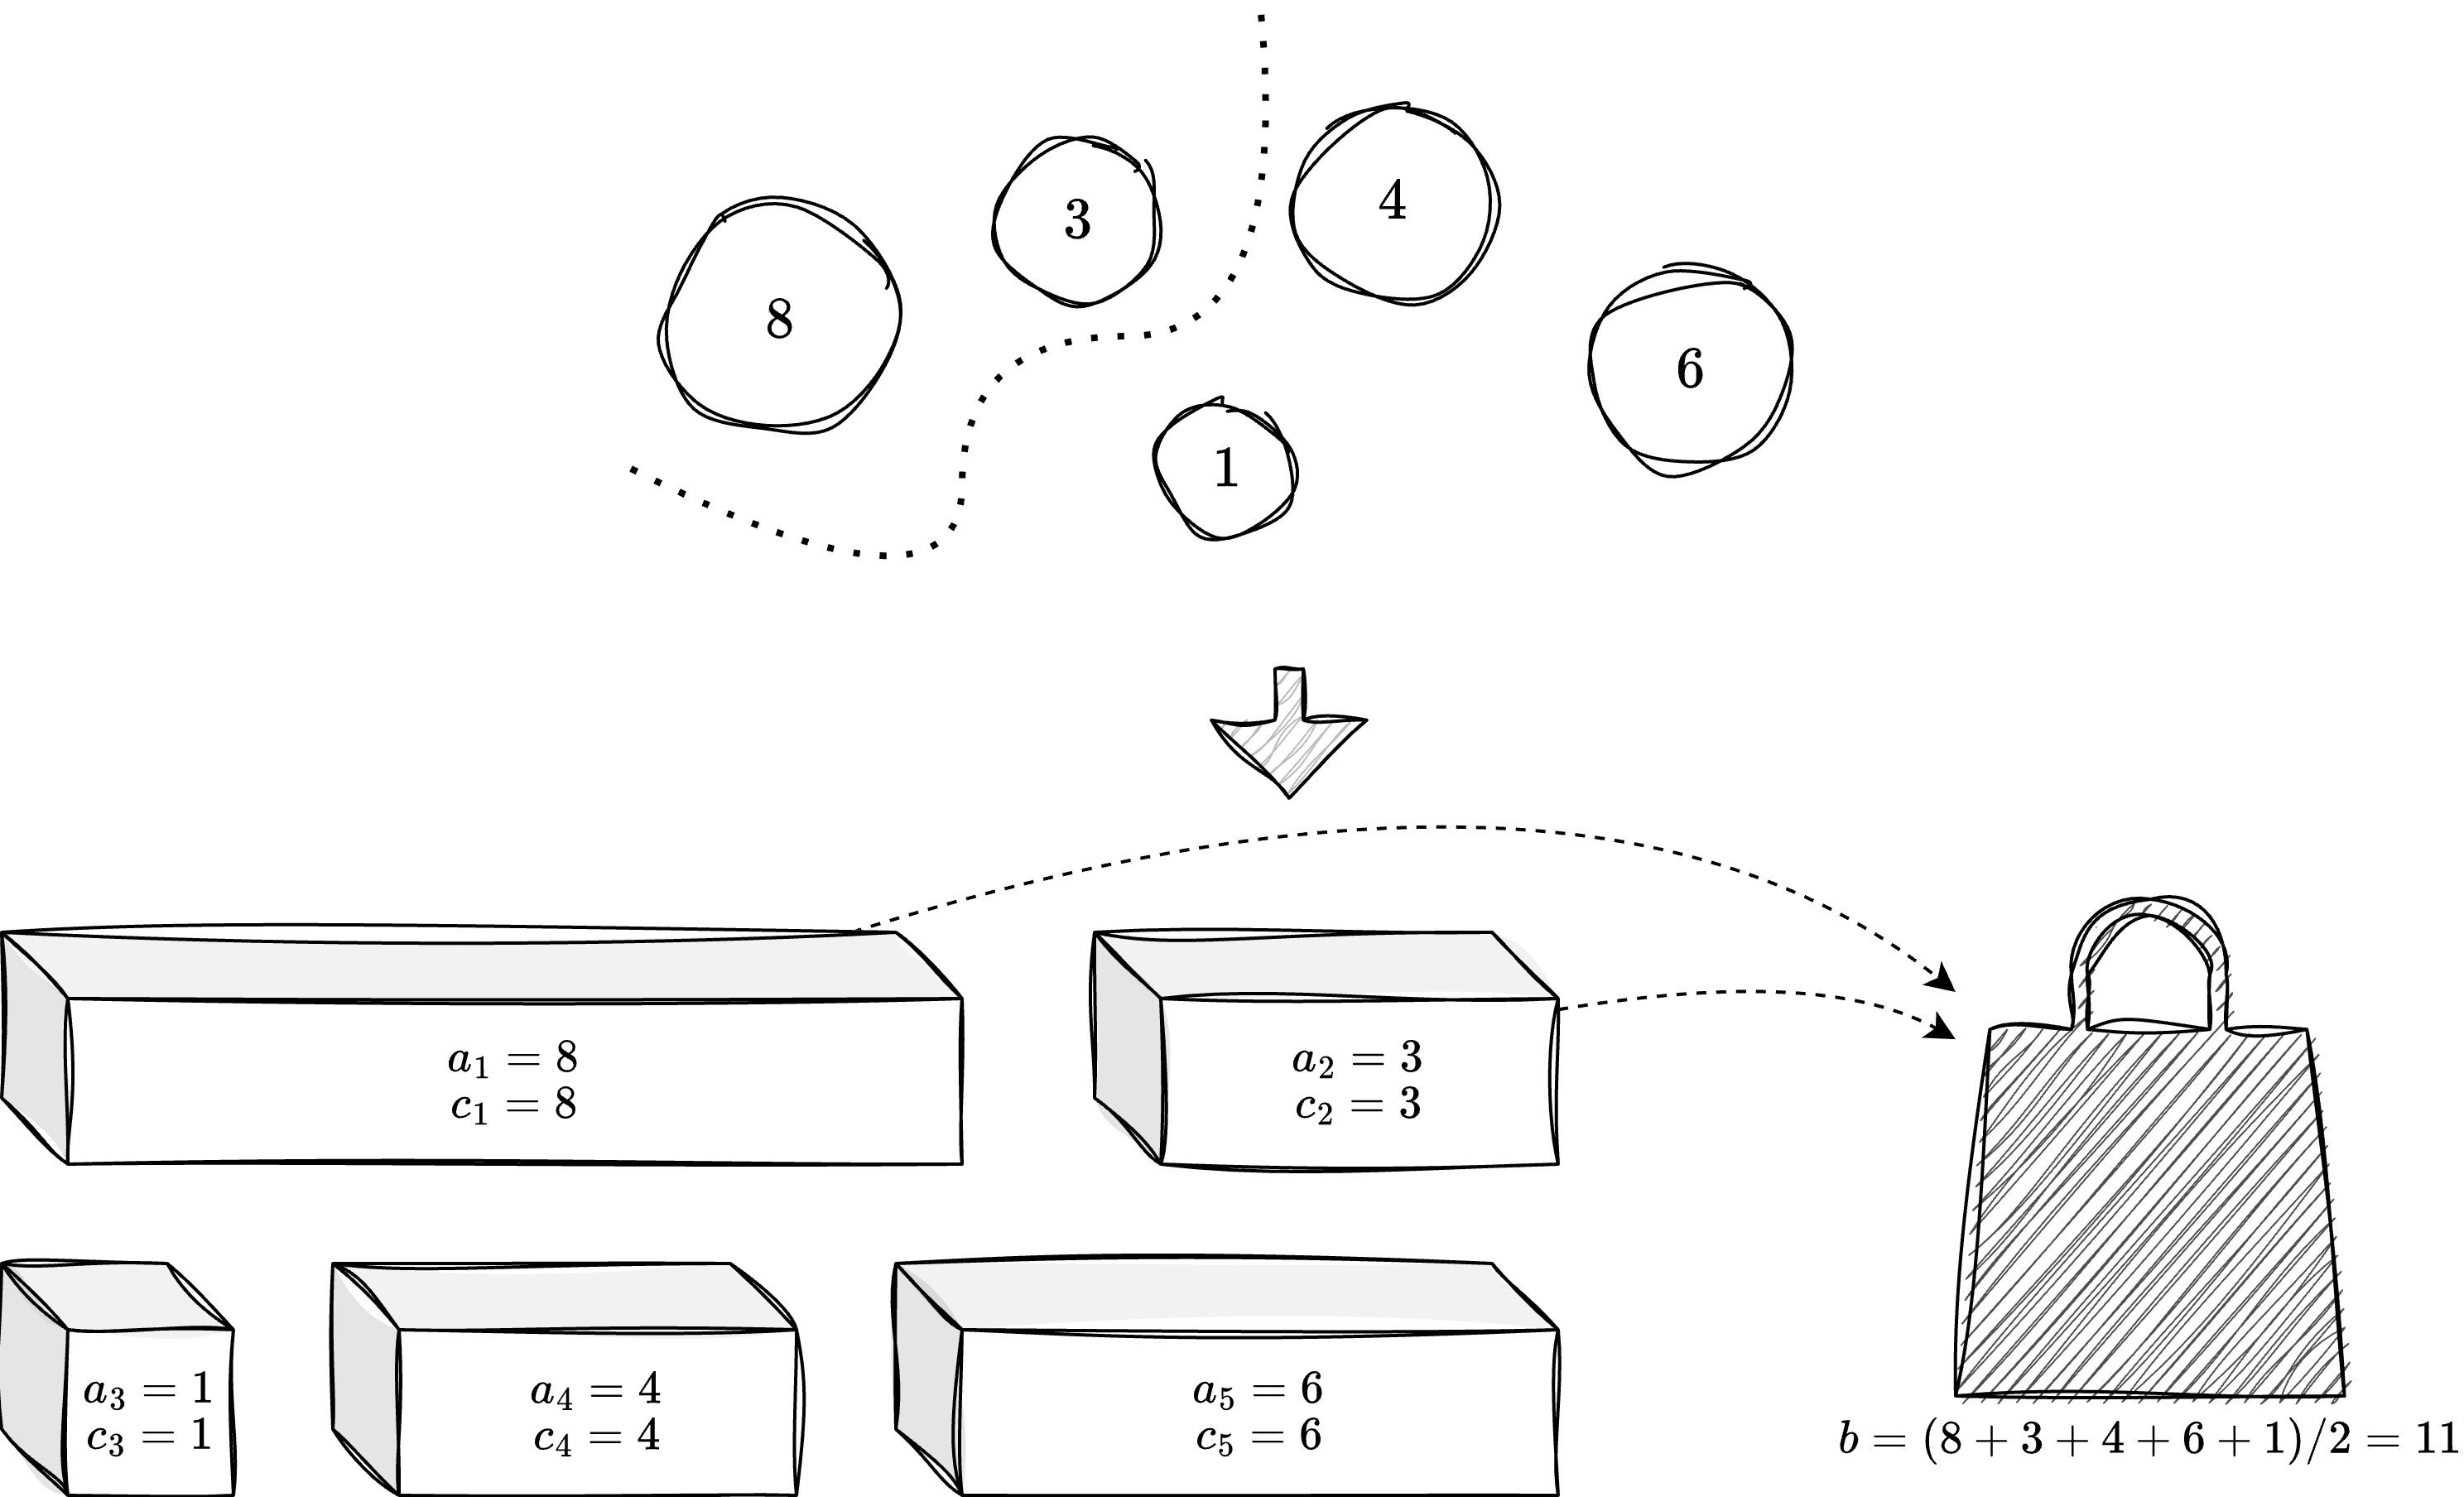
\includegraphics[width=0.8\textwidth]{figures/reduction.png}
	\end{figure}
\end{frame}

\end{document}
